\chapter{A Generative Model of Alzheimer's Disease}
\label{chp:3}

\section{Introduction}
\label{sec:introduction}

We have recently shown that shown that a fully Bayesian pipeline can be used to
calibrate spatiotemporal model of AD \cite{schafer2021bayesian,
schafer2022correlating}. The combination of mechanistic mathematical models and
a full Bayesian analysis is attractive for at least two reasons. First,
mechanistic models allow for interpretation and hypothesis-driven investigation.
Secondly, a Bayesian framework provides a natural and robust method for
comparing models and quantifying uncertainty about model structure and
observations. There is yet to be a fully generative approach to
modelling \TP protein dynamics in the brain that accounts for the observation pipeline 
--- this will be the primary contribution of this chapter.

In this chapter, we use \cref{eqn:fkpp-local} presented in \cref{chp:2} and
hierarchical Bayesian inference to compare population level differences between
groups at different stages of AD progression. The calibrated model fits the data
well and our results highlight two interesting differences between patient
groups. First, there is faster transport early in the disease process. Second,
over the course of the disease there is an acceleration in the accumulation rate
of proteins.

\section{Inference using Patient Data}
\label{sec:inference}

Equipped with a dynamical model of \TP SUVR as a function of \TP concentration
\cref{eqn:fkpp-local}, we seek to apply it to patient data and aim to show how
the model describes AD development in patients. We achieve this using data from
two studies, ADNI, which uses the AV1451 radiotracer, and BioFINDER2 (BF2),
which uses RO948 radiotracer \cite{leuzy2020diagnostic}. Since BF2 data are
collected with a different radiotracer, we reapply the methods described in
\cref{sec:regionalparams} to infer fixed regional parameters, $\mathbf{p_0}$ and
$\mathbf{p_\infty}$ specific to this radiotracer. We then apply Bayesian
inference to estimate the posterior distribution over our model parameters given
patient data. We apply inference to different patient groups given by their \AB
and \TP positivity status and show that there is accelerated proteopathy in
patients with a higher \AB and \TP burden.

\subsection{Data Preparation}

Patient data obtained from ADNI are download as fully processed data, summarised
as SUVR values and volumes for each of the regions in the DKT atlas. For details
on the processing methods used, see \cite{landau2016flortaucipir}. We
re-normalise the values using the inferior cerebellum SUVR reference region.
Data from BF2 was provided to us as fully processed data, also with regional
SUVR values and volumes summarised on the DKT atlas. A detailed account of the
processing methods used in BF2 can be found in \cite{OssenkoppeleRik2018DAo1}.
In both ADNI and BF2, we choose only subjects who have at least three \TP PET
scans, allowing us to perform inference on the time-series model. Demographics 
for the selected ADNI and BF2 subjects are given in \cref{table:demo-adni} and 
\cref{table:demo-bf}, respectively.

\begin{table}[h]
    \centering
    \begin{tabular}{lrrrrrr}
      \hline
      \textbf{Group} & \textbf{Age} & \textbf{\% Female} & \textbf{Education} & \textbf{\% CN} & \textbf{\% MCI} & \textbf{\% AD} \\
      \hline
      \ABP \TPP & 75.8 & 0.63 & 16.59 & 0.44 & 0.37 & 0.19 \\
      \ABP \TPN & 79.1 & 0.39 & 16.87 & 0.57 & 0.39 & 0.04 \\
      \ABN & 73.3 & 0.55 & 17.0 & 0.63 & 0.35 & 0.03 \\\hline
    \end{tabular}
    \caption{Cohort demographics for ADNI.}
    \label{table:demo-adni}
\end{table}

\begin{table}[h]
    \centering
    \begin{tabular}{lrrrrrr}
      \hline
      \textbf{Group} & \textbf{Age} & \textbf{\% Female} & \textbf{Education} & \textbf{\% CN} & \textbf{\% MCI} & \textbf{\% AD} \\
      \hline
      \ABP \TPP & 73.9 & 0.65 & 11.6 & 0.2 & 0.43 & 0.37 \\
      \ABP \TPN & 72.1 & 0.5 & 13.2 & 0.61 & 0.31 & 0.08 \\
      \ABN & 66.9 & 0.5 & 12.8 & 0.81 & 0.19 & 0.0 \\\hline
    \end{tabular}
    \caption{Cohort demographics for BF2.}
    \label{table:demo-bf}
\end{table}

For both datasets, we perform inference over three groups, $A\beta^{-}$,
$A\beta^{+} \tau P^{-}$, $A\beta^{+} \tau P^{+}$. In ADNI, \AB status is
determined by an SUVR cutoff value, given in \cite{landau2016florbetapir}. In
BF2, \AB status is again determined by an SUVR cutoff and reported by individual
scanning sites \cite{ossenkoppele2022amyloid}. We distinguish
between $\tau P^{-}$ and $\tau P^{+}$ using a \TP PET SUVR cut-off for two
composite regions, as detailed in \cite{ossenkoppele2022amyloid} and given in
\cref{table:cutoffs}. There are two cut-offs, one for determining \TP
positivity in the medial temporal lobe (MTL), defined as the mean of four
regions, the bilateral entorhinal and amygdala, and another for cortical
positivity, defined as the middle temporal and inferior temporal gyri. The
thresholds for the composite regions are based on regional Gaussian mixture
models. For each composite region, the SUVR  
threshold is defined as mean of the minimum SUVR values at which each subregion
has a greater than $50\%$ probability of belonging to the \TPP distribution. We
define a subject as being \TPP if their last scan is suprathreshold in either
the MTL or cortical \TP PET SUVR and \TPN if the SUVR value is below both SUVR
thresholds. We use two composite regions for cut-off values to account for 
subjects who have atypical AD, presenting with \TP in the cortrex but not the 
medial temporal lobe \cite{vogel2021four}.

\begin{table}[h]
    \centering
    \begin{tabular}{|l|c|c|}
        \hline
        \textbf{Region} & \textbf{ADNI} & \textbf{BF2}  \\
        \hline
        MTL & $1.375$ & $1.248 $\\
        Cortical & $1.395$ & $1.451$  \\
        \hline
    \end{tabular}
    \caption{SUVR threshold values used for defining \TPP and \TPN subjects}
    \label{table:cutoffs}
\end{table}


\subsection{Probabilistic Model}
For each of the three groups, \ABN, \ABP \TPN, \ABP \TPP, we use a hierarchical
model, factoring over patients and scans. In each group there are $N$ subjects,
each of whom have $T_n$ scans, for $n = 1 \hdots N$ subjects, summarised
over 72 regions, $R = 72$. The observations times, i.e. scan dates, are denoted
by $\mathbf{t} = t^{n}_j$ for $j = 1 \hdots T_n$, $n = 1 \hdots N$. We denote
the full data set for a group as $\mathbf{Y}$ and individual subject data as
$Y^{n}_{ij}$, corresponding to the $n^{th}$ subject, at scan $j = 1 \hdots T_n$
and region $i = 1 \hdots R$. For a single subject, we have the following data 
generating function:
\begin{equation}
    \label{eq:generating-function}
    Y^{n}_{ij} = 
    f_i(\mathbf{y_0}^n, \theta^n, t^n_j) + \epsilon_i.
\end{equation}
where $\mathbf{Y}^{n} \in \mathbb{R}^{R \times T_{n}}$, is the data for the
$n^{th}$ subject, $ \mathbf{y}_0 \in \mathbb{R}^{R}$ are their initial
conditions for $R$ regions, $\theta = \{\rho, \alpha\} \in \mathbb{R}^2$ are
subject model parameters, $\mathbf{t} \in \mathbb{R}^{T_{n}}$ are their
observation times. For the initial conditions, $\mathbf{y}_0$, we use the SUVR
values from the subject's first scan. Ideally, we would assume the initial
conditions are also random variables to be inferred, however this would add $N
\times R$ random variables to the model and make sampling infeasible. To derive
a likelihood function from \cref{eq:generating-function}, we assume the
observations errors are independently and identically distributed and sampled
from a Gaussian distribution with standard deviation $\sigma$. The data
generating distribution for a single observation from a subject is then:
\begin{align}
    \epsilon &\sim \mathcal{N}(0, \sigma^2) \\ 
    Y^{n}_{ij} &\sim \mathcal{N}(f_i(\mathbf{y_0}^n, \theta, t^n_j), \sigma^2)
\end{align}
To extend this to a hierarchical population model, we define random variables,
$\Theta = \{(\rho_i, \alpha_i)\}_{i=1}^{N}$, encoding subject specific model
parameters and hierarchical population parameters, $\Omega = \{ \rho_\mu ,
\rho_\sigma, \alpha_\mu, \alpha_\sigma \}$, upon which each $\Theta_i$ depends.
Additionally, there are fixed parameters $\mathbf{y}_0^n \in \mathbb{R}^{R}$ and
$\mathbf{t}^{n} \in \mathbb{R}^{T_{n}}$ for $n = 1 \hdots N$, encoding each
subject's initial conditions and observations times.
\begin{figure}[H]
    \centering
    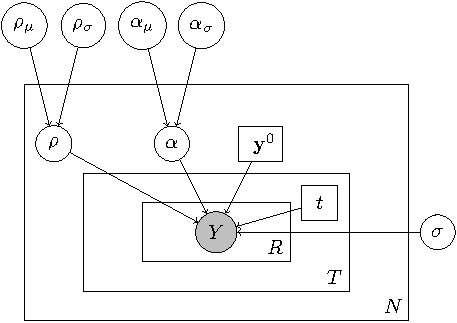
\includegraphics[width=0.75\textwidth]{local-fkpp/inference/plate3.pdf}
    \caption{\textbf{Plate diagram of probabilistic model} showing a graphical
    representation of the hierarchical model used for patient inference.}
    \label{fig:plate}
\end{figure}
A graphical representation of the model is given in \cref{fig:plate}. The
representation of the model as a directed acyclic graph highlights the
conditional dependencies of random variables in the model. From this, we can see
that the likelihood function for a single subject under the hierarchical model
is: 

\begin{equation}
    p(\mathbf{Y}^{n}, \Theta_n \mid \Omega, \sigma, \mathbf{y}_{0}^{n}, \mathbf{t}^{n}) = 
    \prod_j^{T_{n}} \prod_i^R p(Y^{n}_{ij} \mid \Theta_n, \sigma, \mathbf{y}^n_0, t^n_j)
    \,p(\Theta_n \mid \Omega)
\end{equation}
where the first term inside the product on the right hand side is contribution
is the subject level model and the second term is the hierarchical model. The
posterior over hierarchical parameters, subject specific parameters and
observation noise is: 
\begin{equation}
    p(\Theta, \Omega, \sigma \mid \mathbf{Y}, \mathbf{t}, \mathbf{y}_{0})  \propto
    \prod_n^N
    p(\mathbf{Y}^{n}, \Theta_n \mid \Omega, \sigma, \mathbf{y}_{0}^{n}, \mathbf{t}^{n})
    \,p(\Omega, \sigma).
\end{equation}
Next, we perform inference and sample from the posterior distribution to examine 
differences between parameter distributions.


\subsection{Inference over Patient Groups}

\subsection*{Inference Set Up}

We run inference for each patient group separately using a Hamiltonian Monte 
Carlo No-U-Turn Sampler (NUTS). We use the same priors across patient groups; 
these are provided in \cref{table:priors}. We use weakly informative 
priors based on scales at which 
we expect to observe parameter values. The NUTS
sampler is initialised with a unit diagonal Euclidean metric and a target
acceptance ratio of $0.8$. For ADNI data we collected four chains
each with $2000$ samples, and for BF2 data, we collect a single chain of $2000$ 
samples.

\begin{table}[h]
    \centering
    \begin{tabular}{lll}
        \hline
        \textbf{Parameter} & \textbf{Prior} & \textbf{Support} \\
        \hline
        $\rho_\mu$ & $\mathcal{U}(0, 5)$ & $[0, 5]$ \\
        $\rho_\sigma$ & $\Gamma^{-1}(2, 3)$ & $[0, \infty]$ \\
        $\alpha_\mu$ & $\mathcal{U}(-5, 5)$ & $[-5, 5]$ \\
        $\alpha_\sigma$ & $\Gamma^{-1}(2, 3)$ & $[0, \infty]$ \\
        $\rho_i$ & $\mathcal{N}(\rho_\mu, \rho_\sigma)$ & $[0, 5]$ \\
        $\alpha_i$ & $\mathcal{N}(\alpha_\mu, \alpha_\sigma)$ & $[-\infty, \infty]$ \\
        $\sigma$ & $\Gamma^{-}(2,3)$ & $[0, \infty]$\\
        \hline
    \end{tabular}
    \caption{Prior distributions for hierarchical model parameters.}
    \label{table:priors}
\end{table}

\subsection*{Inference Results}

For all patient groups and all chains, we observe good convergence for parameter
distributions in both ADNI and BF2 data. A summary of the hierarchical
parameters is given in \cref{table:pstsummary}. For chain diagnostics, we
report zero divergences in post-warmup samples across all chains, $0.99 \leq
\hat{r} \leq 1.01$, and high effective sample sizes for all parameters.

\subsubsection*{Posterior Distributions}
The hierarchical population parameter distributions are shown in 
\cref{fig:hier-dsts} for ADNI and \cref{fig:hier-dsts-biofinder} for BF2.
There are several interesting observations to be made. First, there is
consistently more uncertainty associated with the \ABN and \ABP \TPN groups,
characterised by the broader distributions for all parameters and higher
parameter values for $\rho_\sigma$ and $\alpha_\sigma$. One contributing factor
to this is the lower signal present in these subjects, increasing the
effect of noise on inference. The higher variance in the \ABP \TPN group may
additionally be explained by higher variance among the subjects, since we only
classify subject inclusion in \TPP or \TPN based on their SUVR relative to the
cut-off values (\cref{table:cutoffs}). It does not take into account
subjects who have have a positive trajectory in \TP SUVR and might have or later
develop tau pathology.

\begin{table}[H]
    \centering
    \begin{tabular}{|r|rr|rr|rr|rr|}
      \hline
      \multirow{2}{*}{\textbf{Group}} &
        \multicolumn{2}{c|}{$\rho_\mu$} &
        \multicolumn{2}{c|}{$\rho_\sigma$} &
        \multicolumn{2}{c|}{$\alpha_\mu$} &
        \multicolumn{2}{c|}{$\alpha_\sigma$} \\
      & mean & s.d. & mean & s.d. & mean & s.d. & mean & s.d.  \\
      \hline
      \ABP \TPP & $0.0357$ & $0.0317 $ & $0.2965$ & $0.0544$ & $0.1277$ & $0.0359$ & $0.1856$ & $0.0309$  \\

      \ABP \TPN & $0.1871$ & $0.1514$ & $0.8076$ & $0.1787$ & $-0.0520$ & $0.1003$ & $0.4248$ & $ 0.0796$ \\

      \ABN & $0.0616$ & $0.0543$ & $0.4780$ & $0.0838$ & $-0.1346$ & $0.0504$ & $0.2937$  & $ 0.0446 $ \\
      \hline
    \end{tabular}
    \caption{\textbf{Posterior Summary: ADNI} Means of hierarchical population parameters.}
    \label{table:pstsummary}
\end{table}

\begin{table}[H]
    \centering
    \begin{tabular}{|r|rr|rr|rr|rr|}
      \hline
      \multirow{2}{*}{\textbf{Group}} &
        \multicolumn{2}{c|}{$\rho_\mu$} &
        \multicolumn{2}{c|}{$\rho_\sigma$} &
        \multicolumn{2}{c|}{$\alpha_\mu$} &
        \multicolumn{2}{c|}{$\alpha_\sigma$} \\
      & mean & s.d. & mean & s.d. & mean & s.d. & mean & s.d.  \\
      \hline
      \ABP \TPP & $0.0114$ & $0.0107$ & $0.1693$ & $ 0.0235$ & $0.1104 $ & $0.0167$ & $0.1202$ & $0.0143$  \\

      \ABP \TPN & $0.2726$ & $0.2430$ & $1.5019$ & $0.4574$ & $0.0142$ & $0.0613$ & $0.2687$ & $0.0513$ \\

      \ABN & $0.0700$ & $0.0697$ & $1.1070$ & $0.1475$ & $-0.0569$ & $0.0314$ & $0.2131$  & $0.0259$ \\
      \hline
    \end{tabular}
    \caption{\textbf{Posterior Summary: BF2}    Means of hierarchical population parameters.}
    \label{table:pstsummary-bf}
\end{table}

The posterior distributions also inform us on the global dynamical regimes
across different stages of AD progression, where a diffusion dominated regime is
given when $ \rho \ll \alpha $, form and a growth dominated regime when $ \rho
\gg \alpha$ (in dimensionless form). The dimensionless parameters are given in
\cref{table:pstsummary} for ADNI \cref{table:pstsummary-bf} for BF2.
In both datasets the inferred parameters suggest that the transport of toxic
proteins in \ABN and \ABP \TPP are decay/growth dominated, $ \rho_\mu \ll
\alpha_\mu $, but in \ABP \TPP it is diffusion dominated $ \rho_\mu \gg
\alpha_\mu $. This suggests that during early disease, proteins are transported
around the brain network more than in later stage AD, where pathology is
primarily driven by growth, as evidenced by the higher growth parameter in the
\ABP \TPP group.

Lastly, the growth parameter increases depending on the AD group, from \ABN to
\ABP \TPN and finally to \ABP \TPP. This result has two implications. First, AD
pathology depends on the presence of toxic \AB, evident by the positive growth
rates estimated in the \ABP groups and predominantly negative growth in the \ABN
group. Secondly, as AD progresses, there is an acceleration of toxic \TP
accumulation, seen by the increased growth rates of toxic \TP in the \ABP \TPP
group compared to the \ABP \TPN group.

\begin{figure}[H]
    \centering
    \begin{subfigure}{0.8\textwidth}
        \centering
        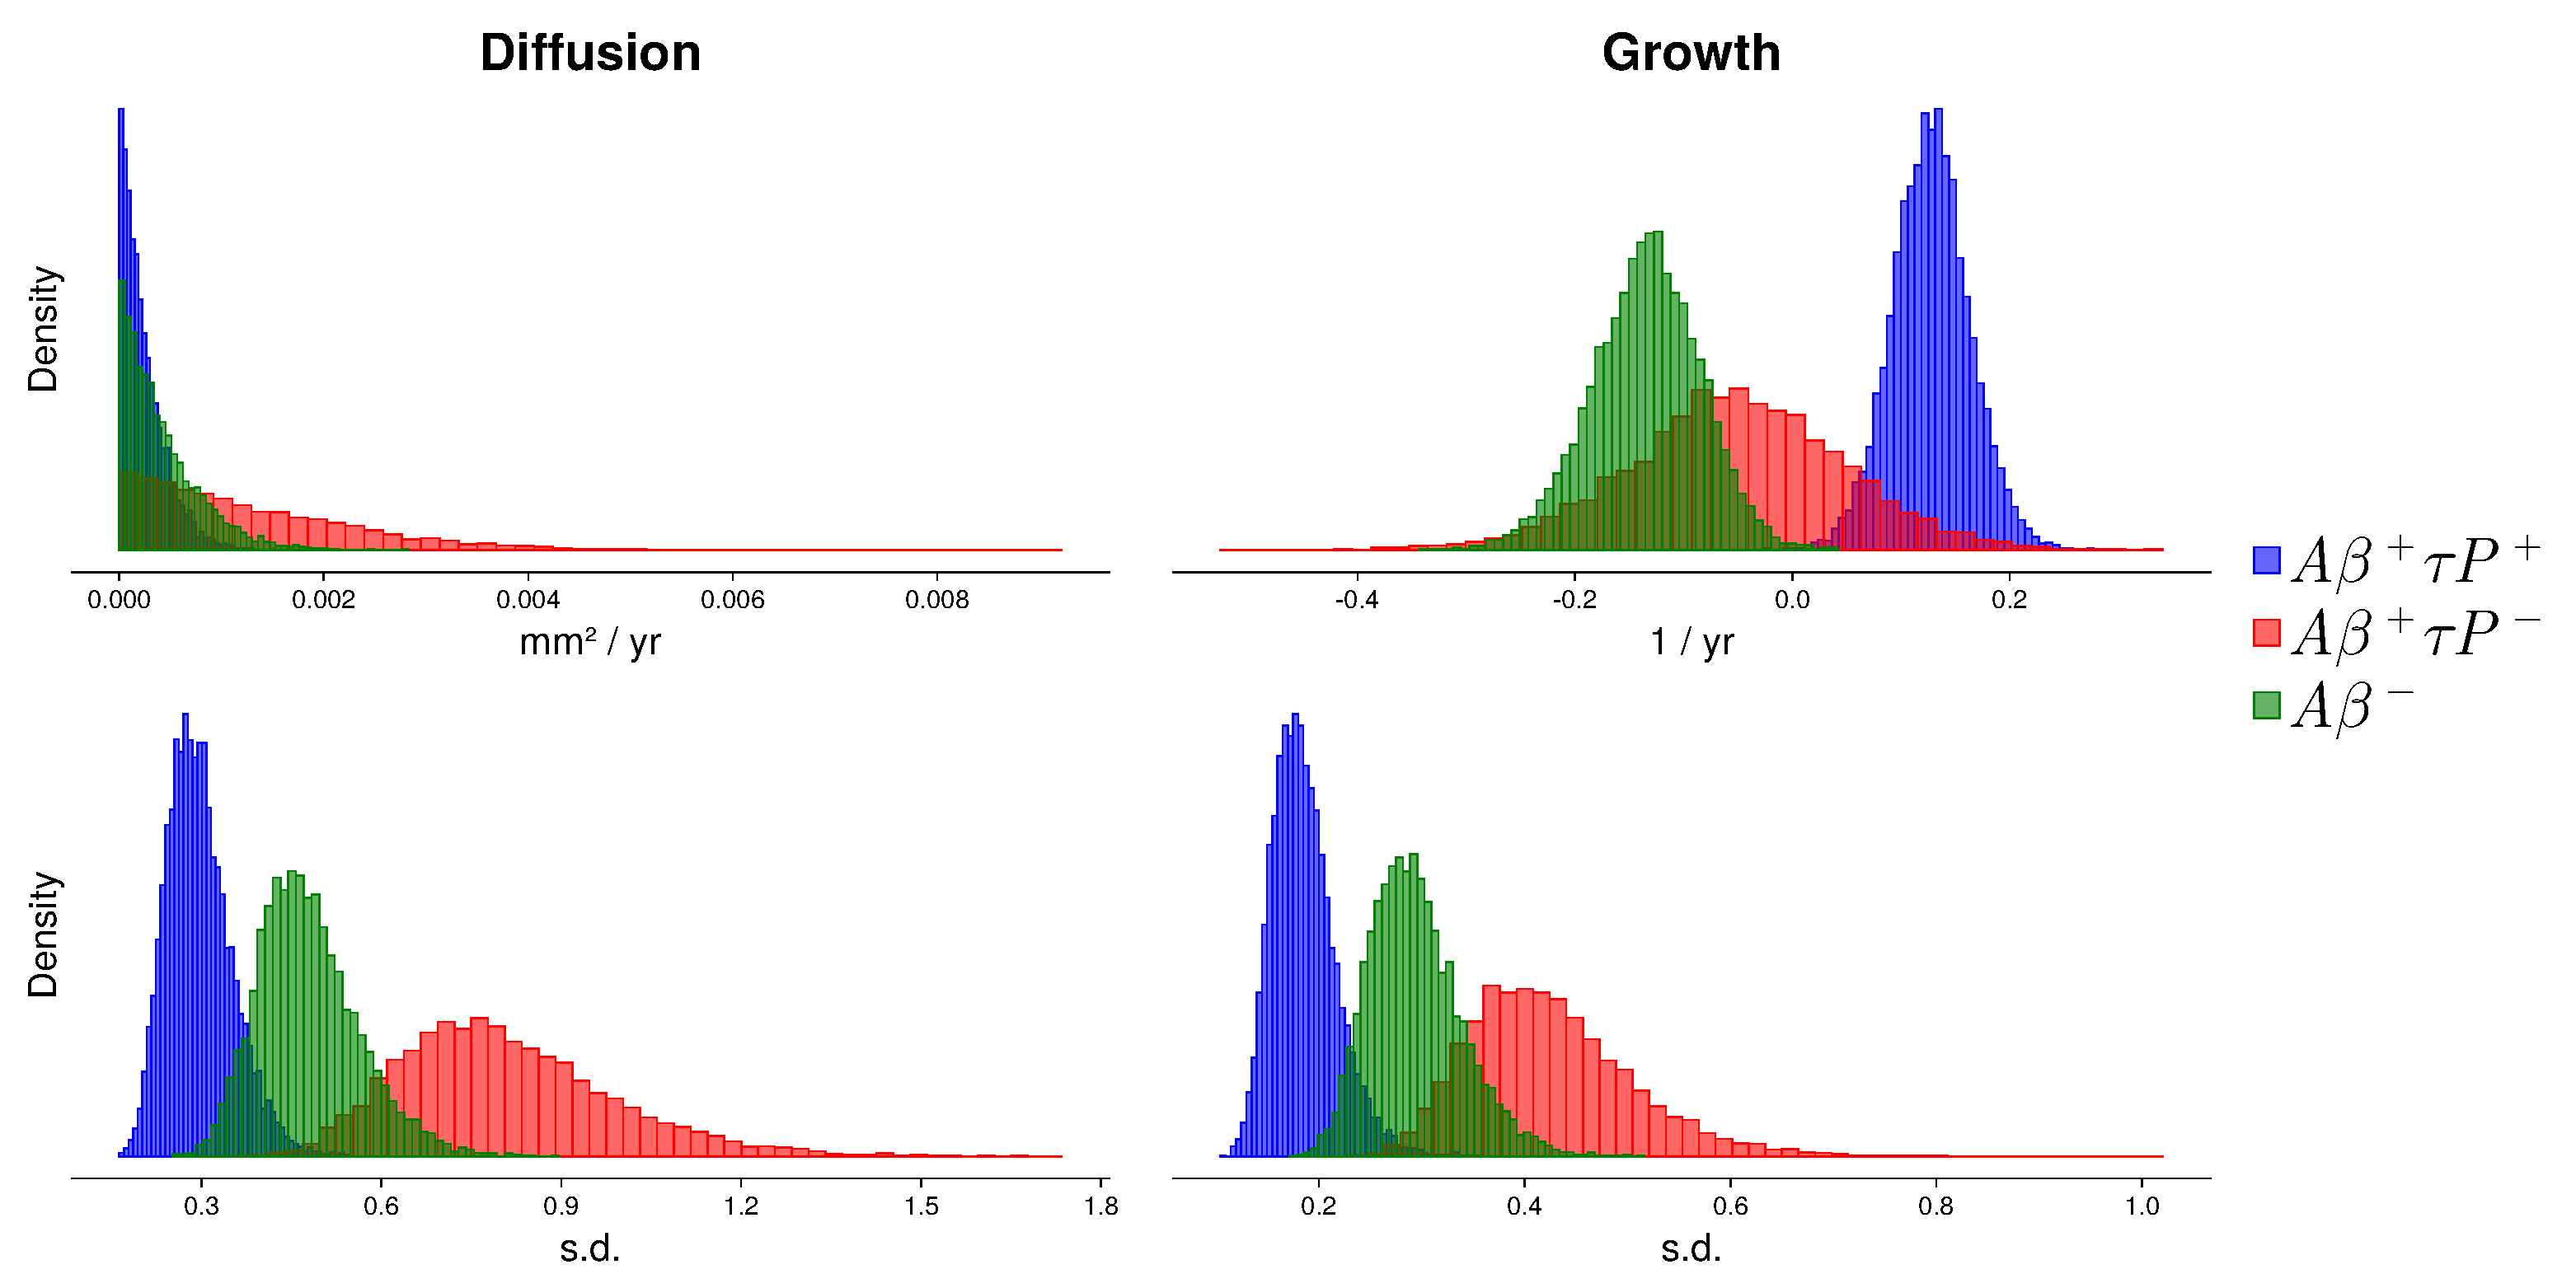
\includegraphics[width=\textwidth]{local-fkpp/inference/hier-dsts.pdf}
        \caption{Distributions of hierarchical population model parameters.}
        \label{fig:hier-dsts}
    \end{subfigure}

    \begin{subfigure}{0.8\textwidth}
        \centering
        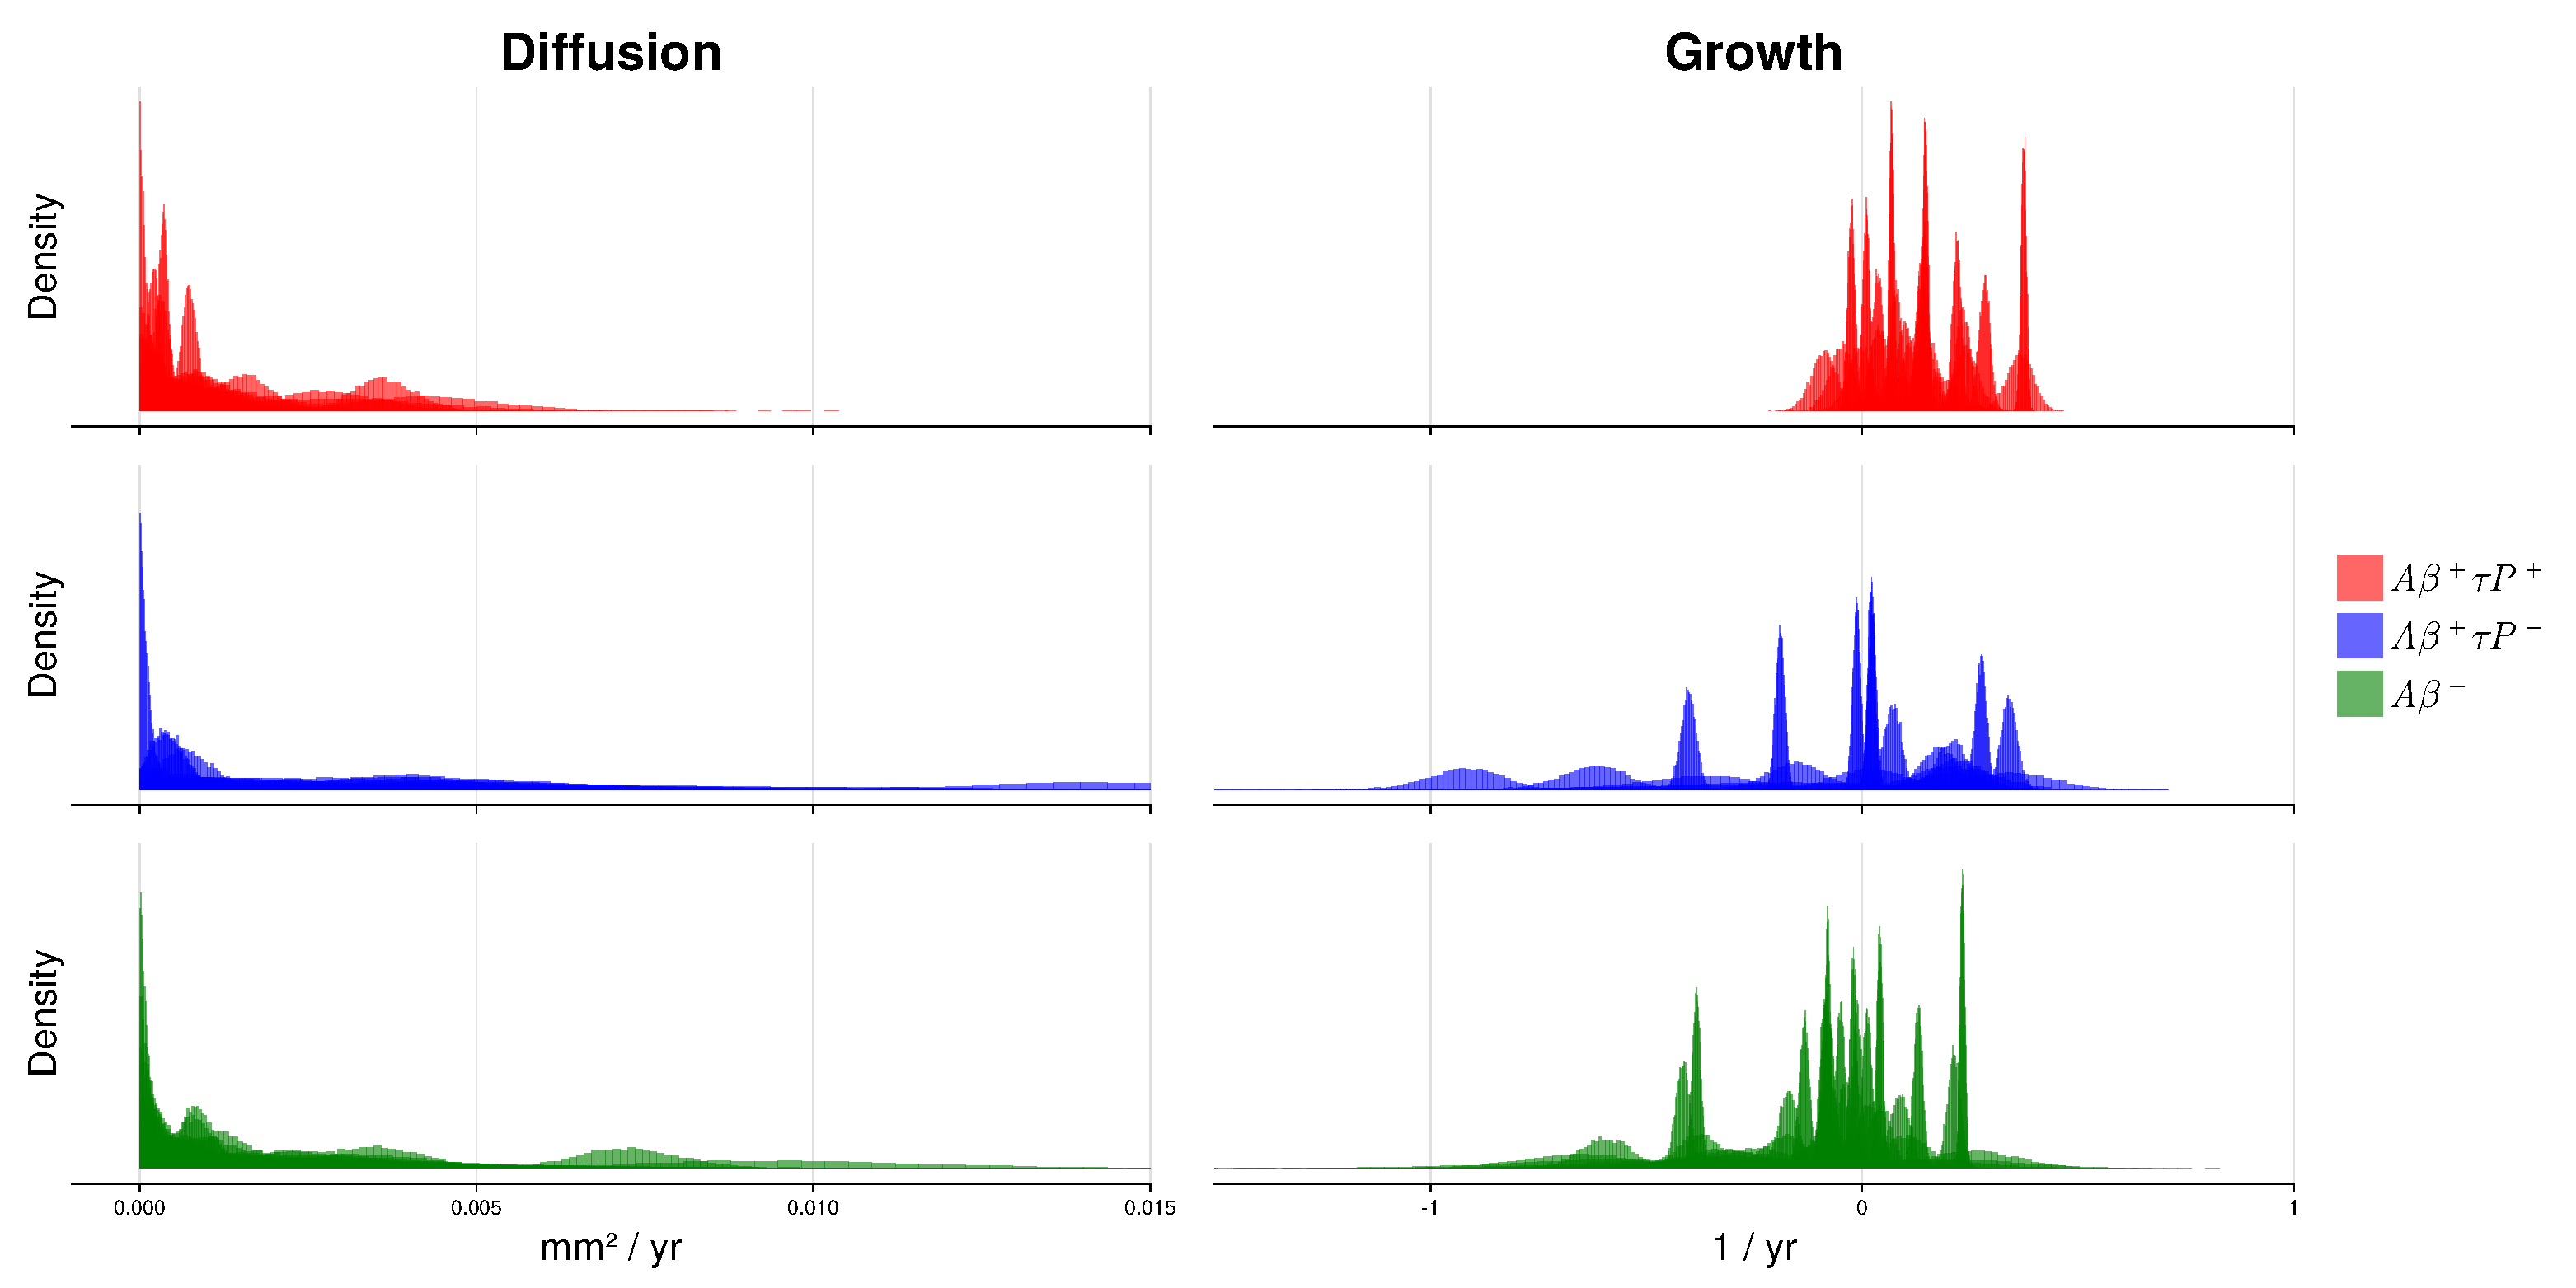
\includegraphics[width=\textwidth]{local-fkpp/inference/sub-dsts.pdf}
        \caption{Distributions of individual model parameters.}
        \label{fig:sub-dsts}
    \end{subfigure}
    
    \caption{\textbf{Posterior distributions from ADNI data.} 
    Inferred posterior distributions for hierarchical population model
    parameters and individual model parameters.}
    \label{fig:inferred-dsts}
\end{figure}

\begin{figure}[H]
    \centering
    \begin{subfigure}{\textwidth}
        \centering
        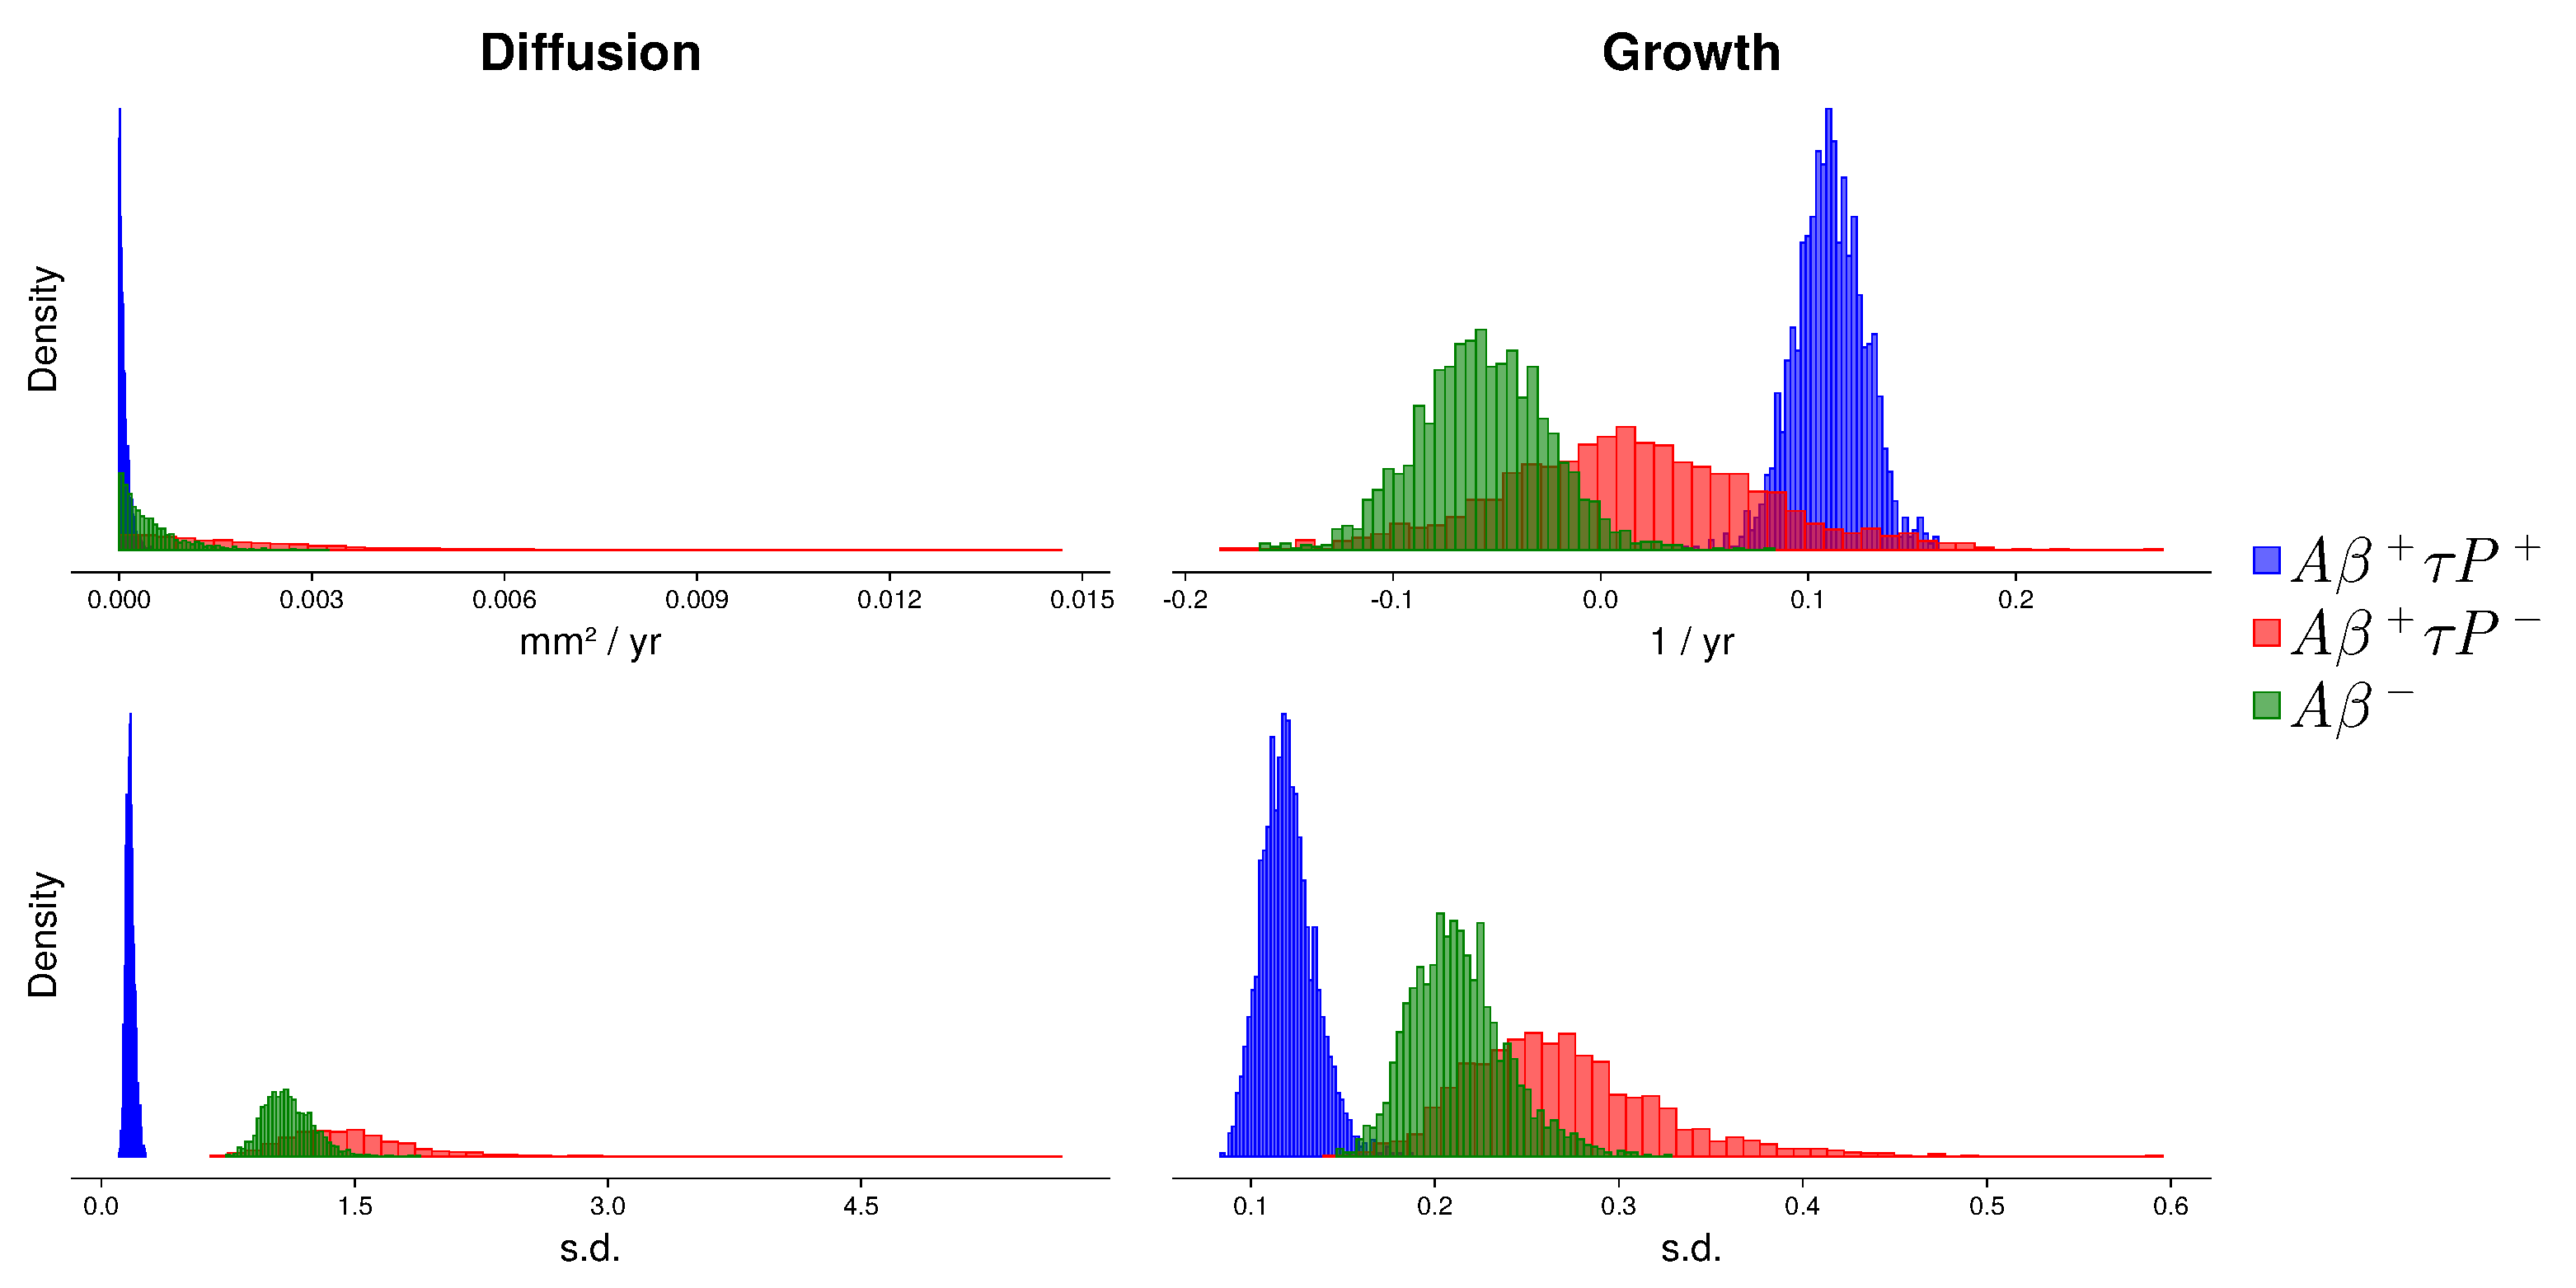
\includegraphics[width=\textwidth]{biofinder/hier-dsts-2000-fd-065-c99.pdf}
        \caption{Distributions of hierarchical population model parameters.}
        \label{fig:hier-dsts-biofinder}
    \end{subfigure}

    \begin{subfigure}{\textwidth}
        \centering
        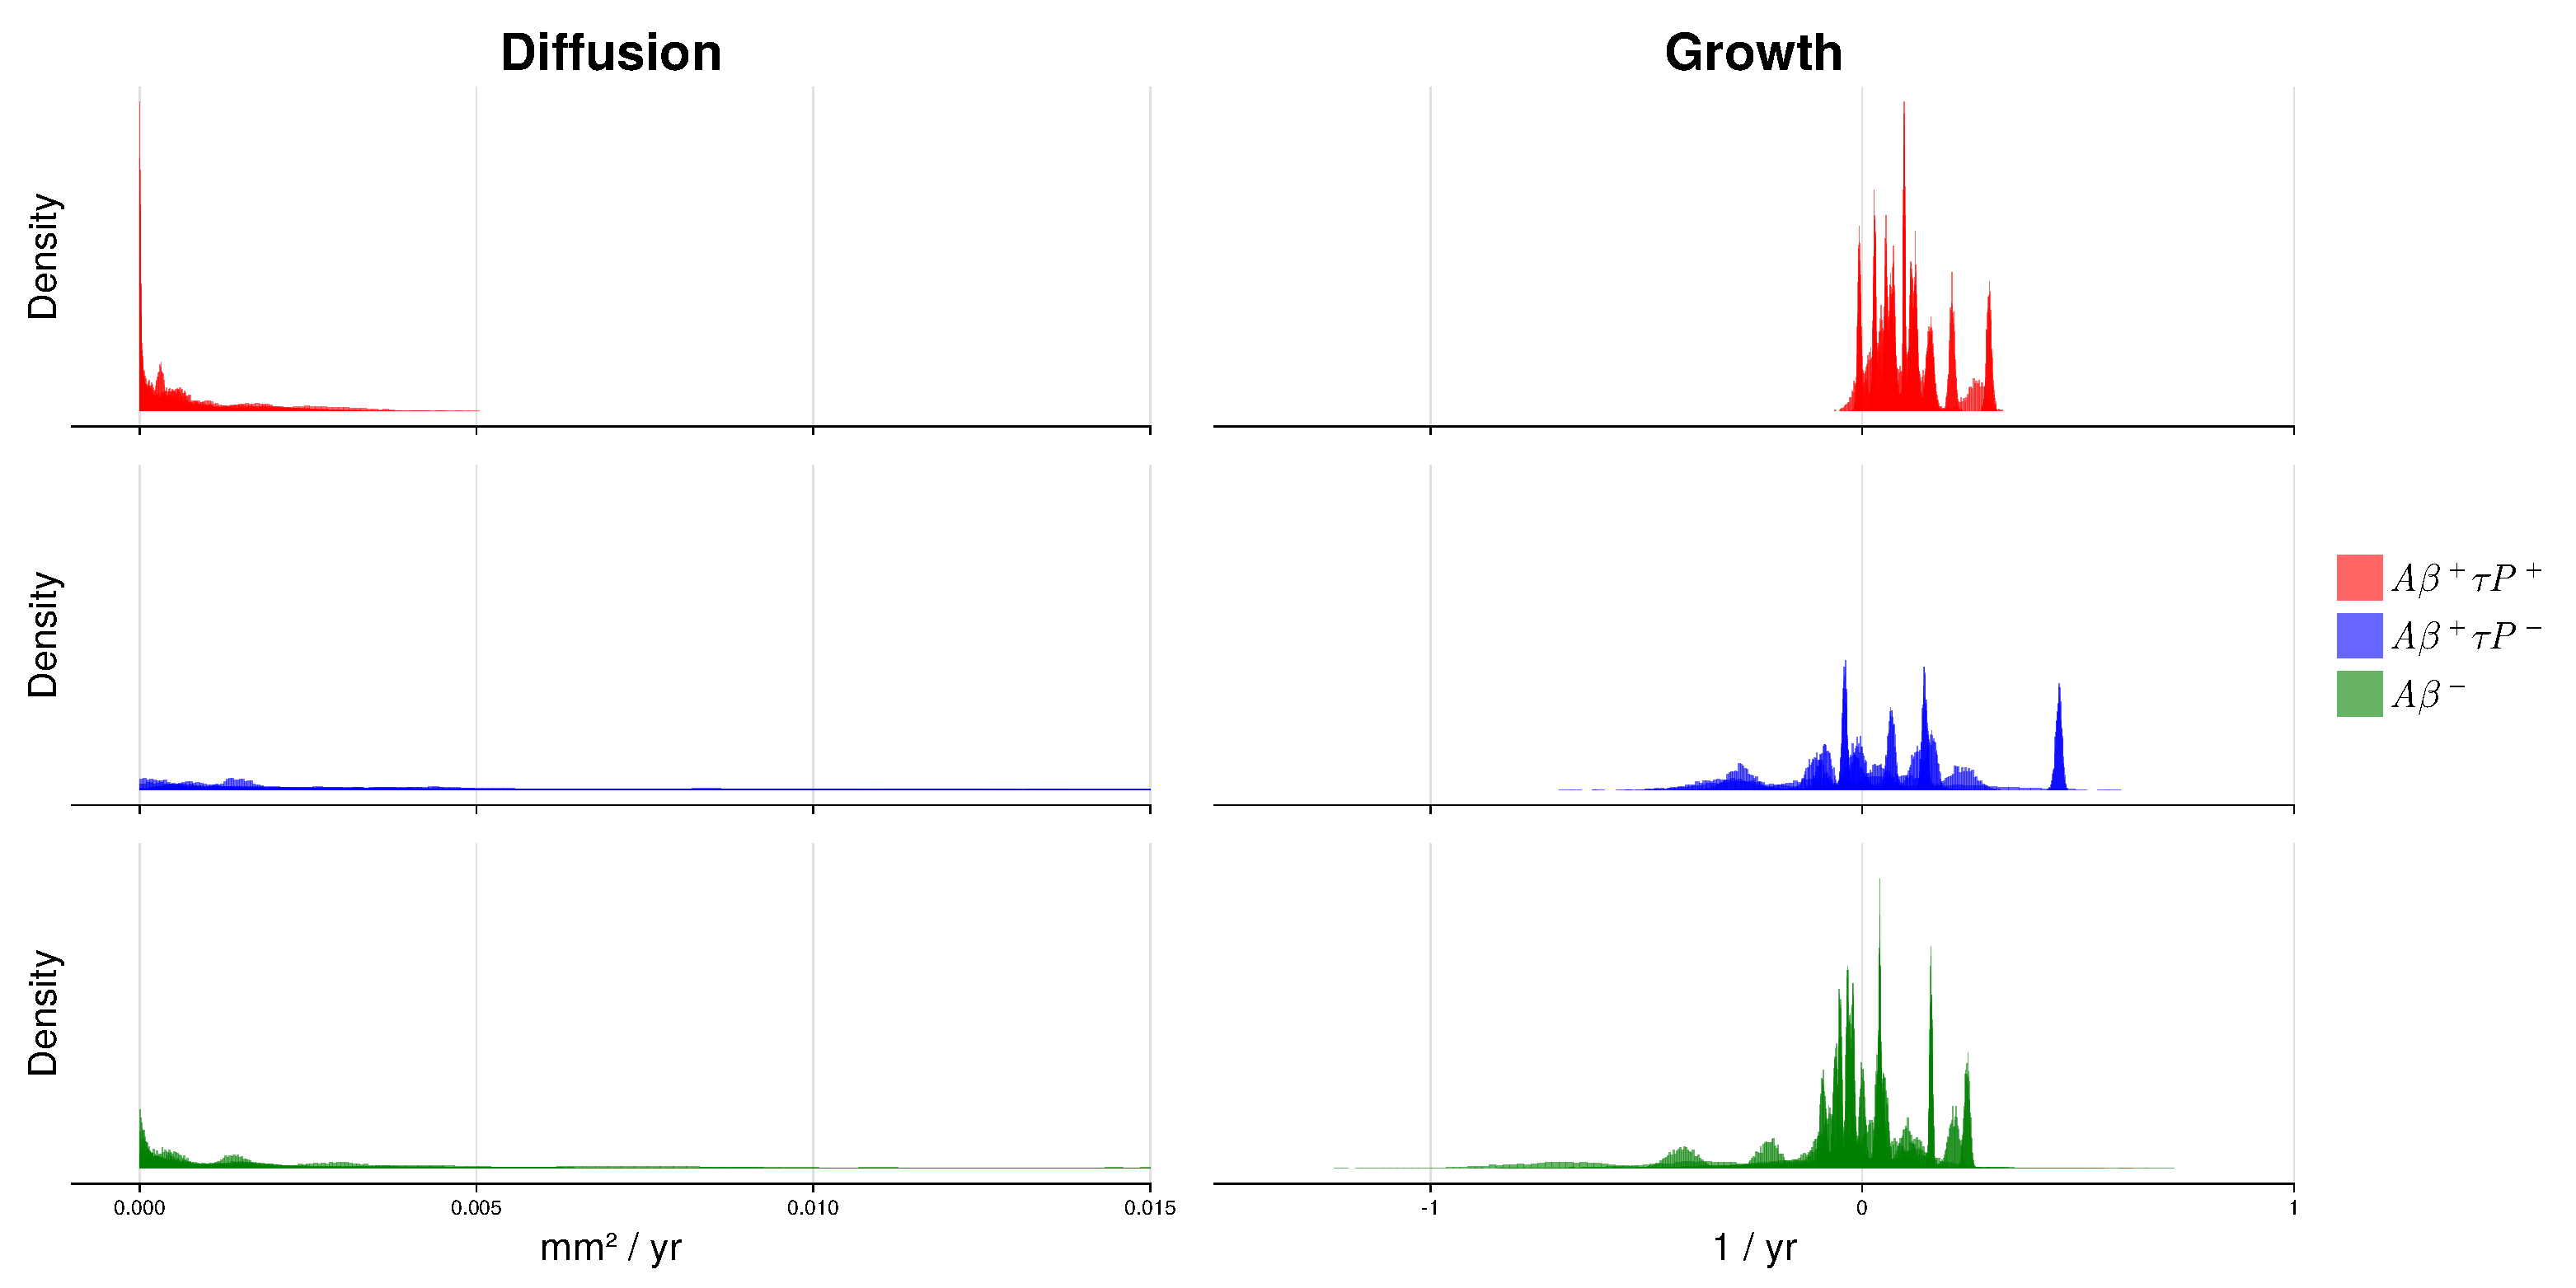
\includegraphics[width=\textwidth]{biofinder/sub-dsts-2000-fd-065-c99.pdf}
        \caption{Distributions of individual model parameters.}
        \label{fig:sub-dsts-biofinder}
    \end{subfigure}
    
    \caption{\textbf{Posterior distributions from BF2.} 
    Inferred posterior distributions for hierarchical population model
    parameters and individual model parameters.}
    \label{fig:inferred-dsts-biofinder}
\end{figure}

\subsubsection*{Posterior Predictive Simulations}

Using the posterior distributions, we can generate samples from the posterior
predictive distributions to assess the goodness of fit and uncertainty in
predictions. Simulations from the \TPP group are shown in
\cref{fig:pstpred-taupos-it,fig:pstpred-taupos-ec} for ADNI, showing data and
simulations from the right inferior temporal lobe and right entorhinal cortex,
respectively, and \cref{fig:pstpred-taupos-it-bf,fig:pstpred-taupos-ec-bf} for
BF2. Similarly, simulations from the \TPN group are shown in
\cref{fig:pstpred-tauneg-it,fig:pstpred-tauneg-ec} for ADNI, and
\cref{fig:pstpred-tauneg-it-bf,fig:pstpred-tauneg-ec-bf} for BF2. Generally, the
calibrated models fit the data very well, and it can be seen that the \TPP
subjects typically have disease progression, whereas \TPN subjects are more
likely to decline, remain stable, or increase more slowly and with greater
uncertainty. 

There are some data points that are not captured within the confidence
intervals. There are a few reasons why data points might not be captured by the
calibrated model. First, we have used a hierarchical model to group information
across subjects and to limit over-fitting through shrinkage, this includes
grouping together observation noise into a single noise parameter. Secondly,
although we have used some regional information in the form of local \p0 and \pI
values, we still have a global growth parameter, $\alpha$, which may prevent
regional trajectories from capturing data points so as to maximise the fit
across all regions. Thridly, we have not incorporated uncertainty around the
initial conditions, which are taken as the SUVR values at the first observation.
This introduces potentially large variations into the forward simulations and
could account for some data points not being captured. Finally, our model is
incapable of describing non-monotonic trajectories and therefore cannot capture
variations in data that might be explained by short-time fluctuations in \TP
concentration, due to clearance or volume atrophy. An example of this can be
seen in the bottom left image of \cref{fig:pstpred-taupos-ec}, where there is a
marked decline in SUVR but increase in the right inferior temporal lobe of same
subject in \cref{fig:pstpred-taupos-it}. Given that the SUVR value in the
entorhinal cortex is close to the carrying capacity, this is likely due to
atrophy of the entorhinal cortex, known to be among the first regions to
degenerate, and therefore a decreasing SUVR. Future work should aim to address 
these limitations, particularly those stemming from simplifying assumptions, to 
provide a more complete method for predicting single subject trajectories.

\begin{figure}[H]
    \centering
    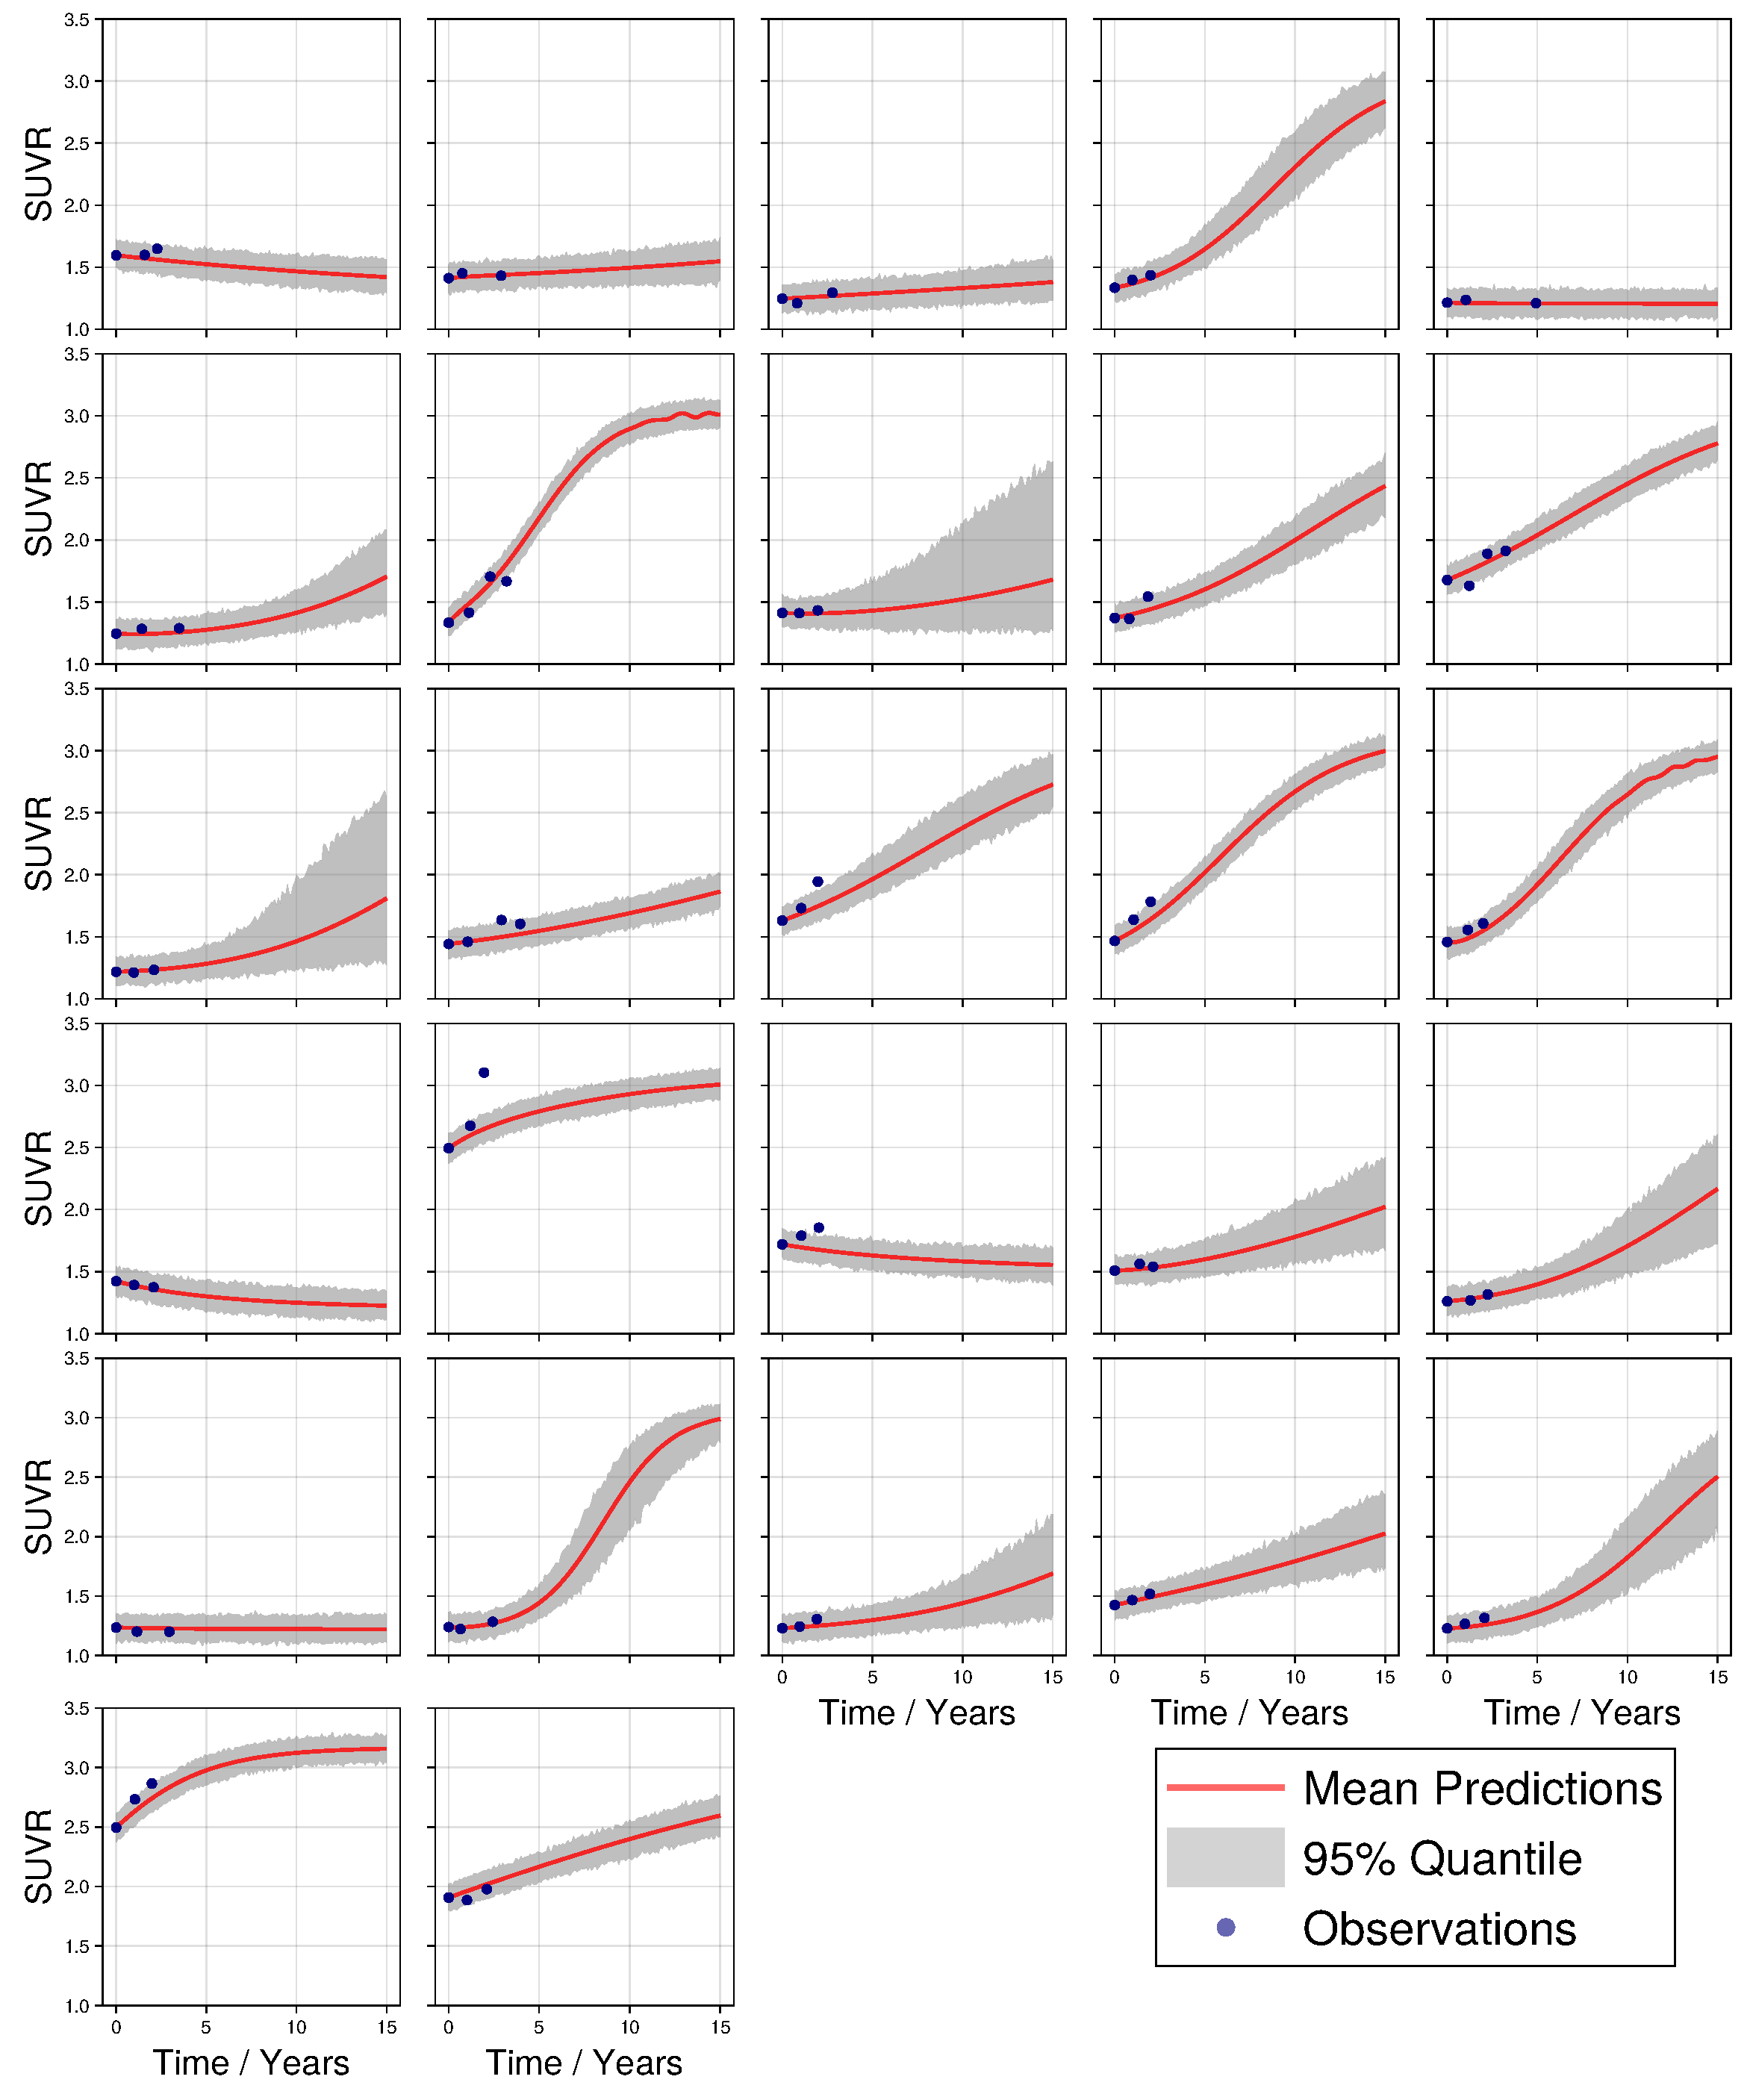
\includegraphics[width=1.0\textwidth]{local-fkpp/inference/pstpred-taupos-inferiortemporal.pdf}
    \caption{\textbf{Posterior predictive trajectories for the right inferior
    temporal lobe in ADNI \ABP \TPP}Forward simulations from the posterior
    distributions of the \TPP group. Shown here are data (blue scatter points)
    and simulated trajectories (mean predictions in red and 95\% confidence
    intervals in grey) from the right inferior temporal lobe.}
    \label{fig:pstpred-taupos-it}
\end{figure}

\begin{figure}[H]
    \centering
    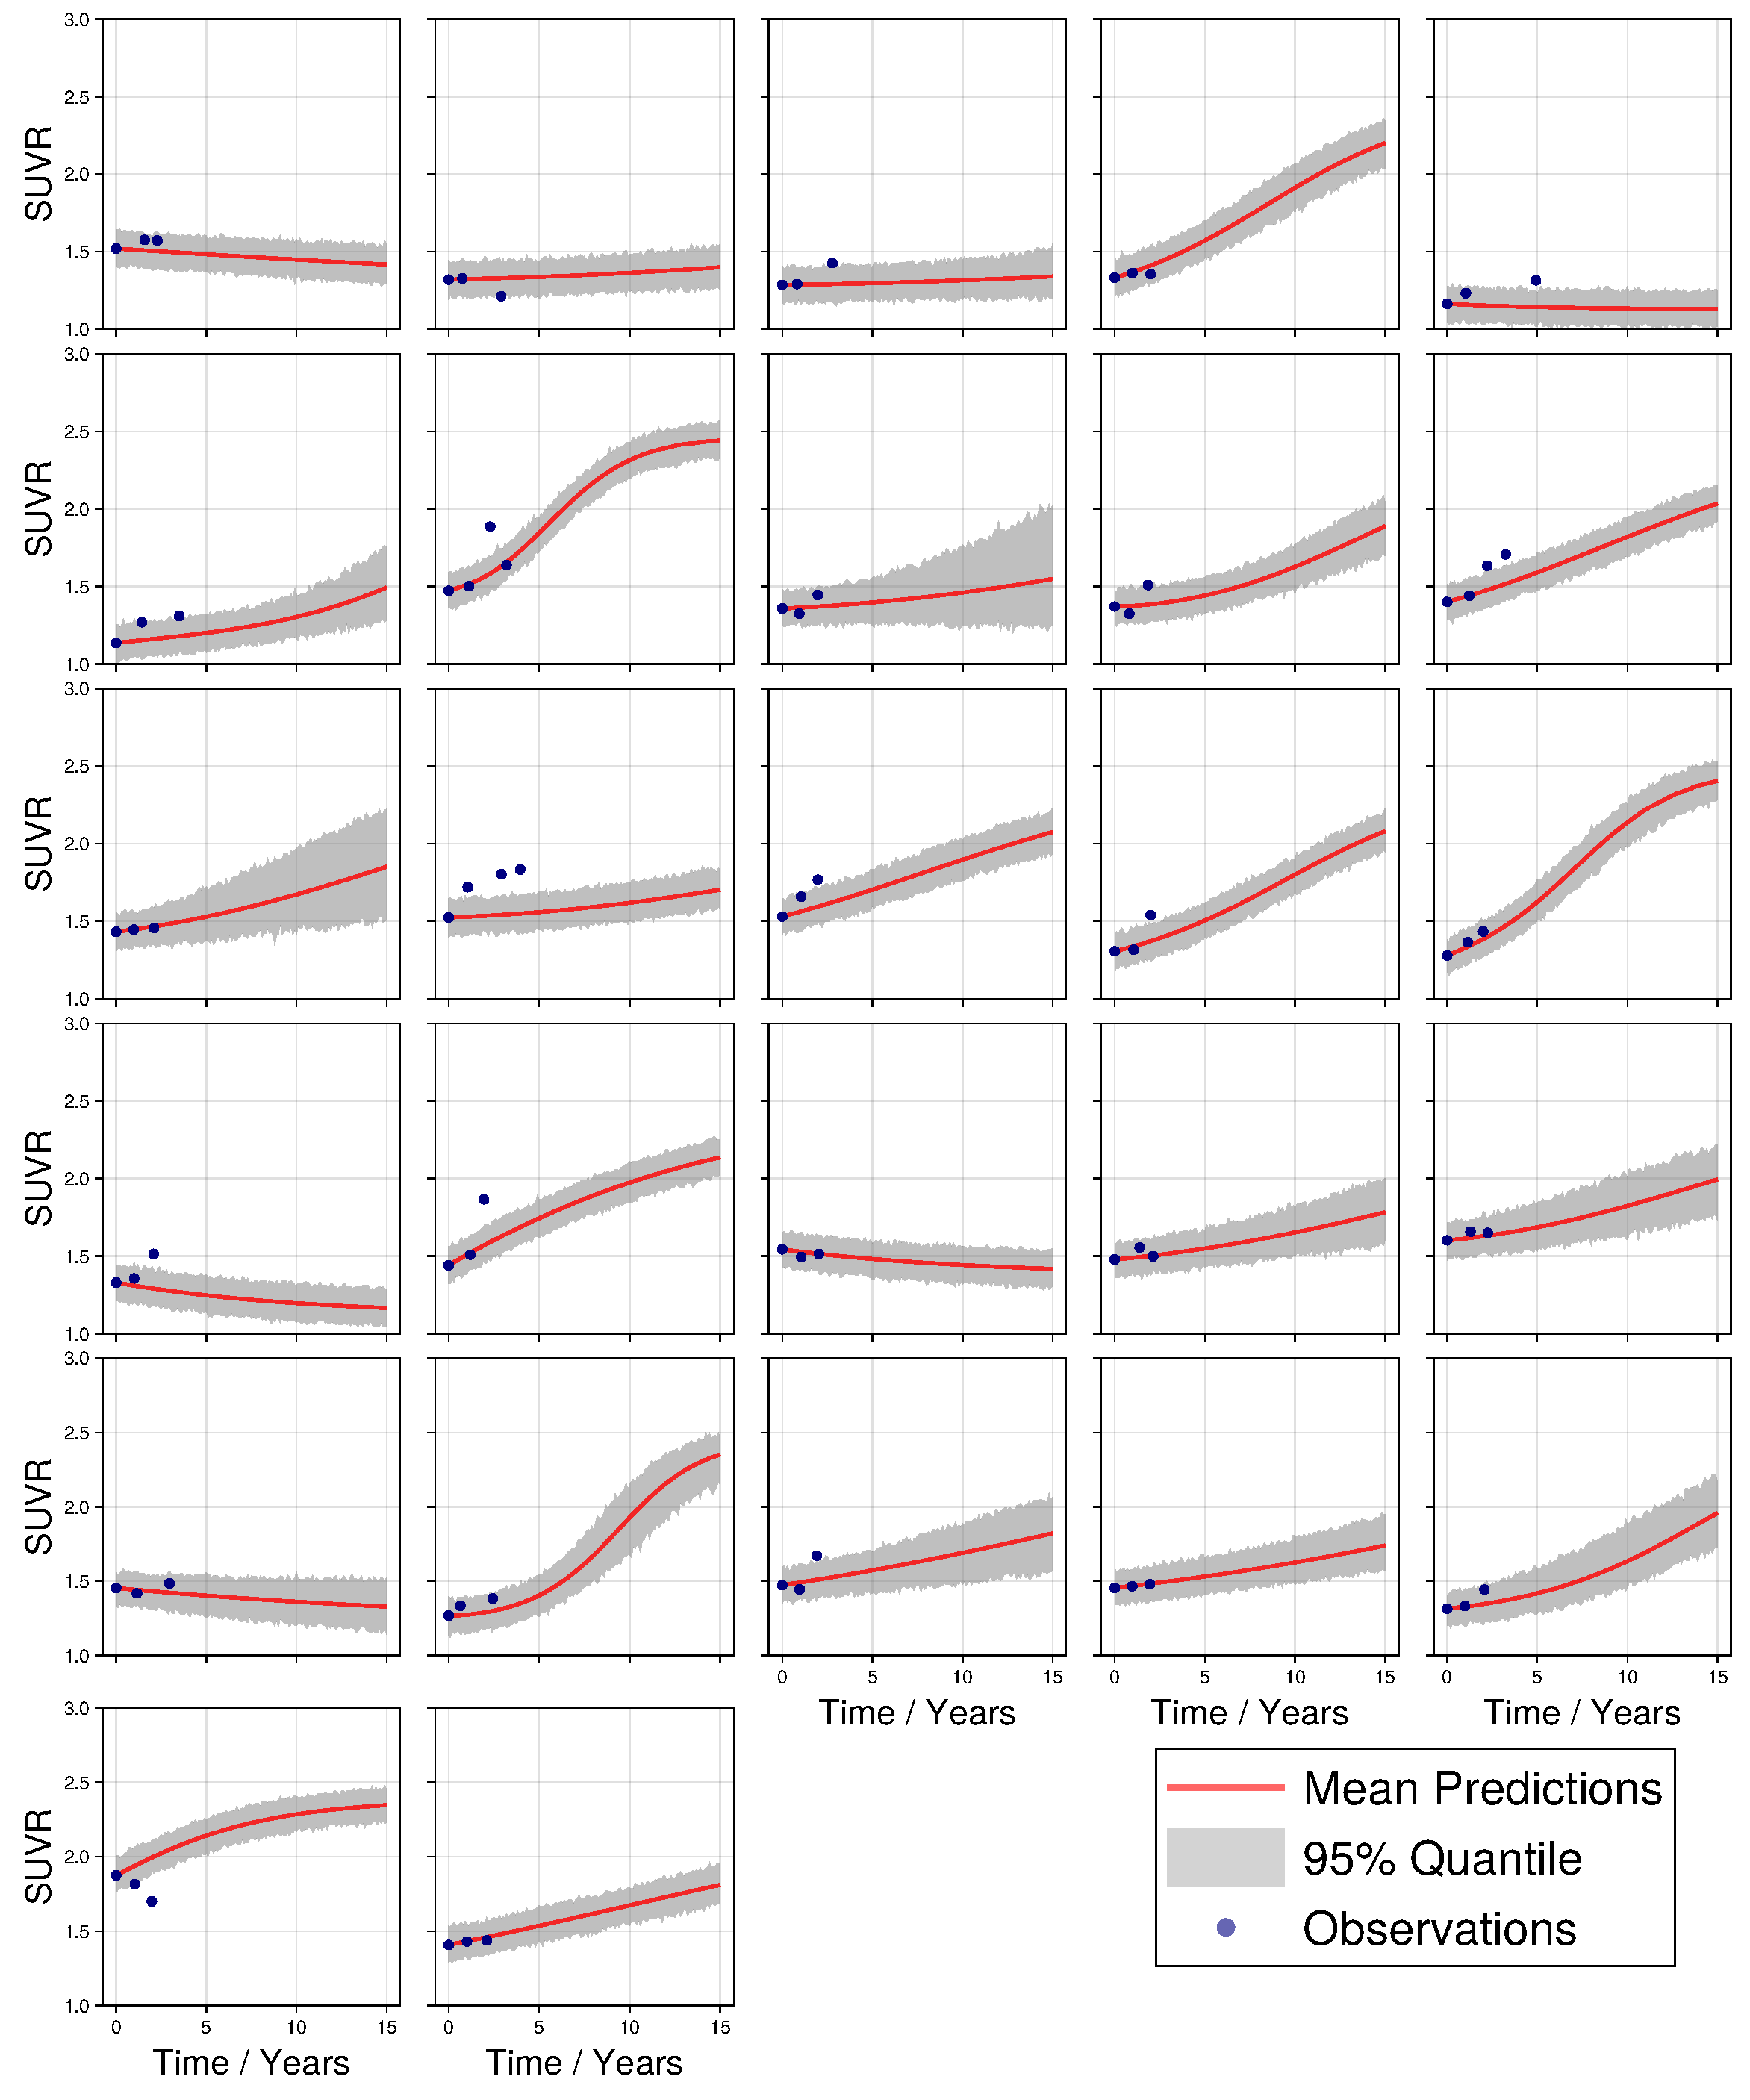
\includegraphics[width=1.0\textwidth]{local-fkpp/inference/pstpred-taupos-entorhinal.pdf}
    \caption{\textbf{Posterior predictive trajectories for the right entorhinal
    cortex in ADNI \ABP \TPP}Forward simulations from the posterior
    distributions of the \TPP group. Shown here are data (blue scatter points)
    and simulated trajectories (mean predictions in red and 95\% confidence
    intervals in grey) from the right entorhinal cortex.}
    \label{fig:pstpred-taupos-ec}
\end{figure}

\begin{figure}[H]
    \centering
    \includegraphics[width=1.0\textwidth]{local-fkpp/inference/pstpred-tauneg-inferiortemporal.pdf}
    \caption{\textbf{Posterior predictive trajectories for the right inferior
    temporal lobe in ADNI \ABP \TPN}Forward simulations from the posterior
    distributions of the \TPN group. Shown here are data (blue scatter points)
    and simulated trajectories (mean predictions in red and 95\% confidence
    intervals in grey) from the right inferior temporal lobe.}
    \label{fig:pstpred-tauneg-it}
\end{figure}

\begin{figure}[H]
    \centering
    \includegraphics[width=1.0\textwidth]{local-fkpp/inference/pstpred-tauneg-entorhinal.pdf}
    \caption{\textbf{Posterior predictive trajectories for the right entorhinal
    cortex in ADNI \ABP \TPN}Forward simulations from the posterior
    distributions of the \TPN group. Shown here are data (blue scatter points)
    and simulated trajectories (mean predictions in red and 95\% confidence
    intervals in grey) from the right entorhinal cortex.}
    \label{fig:pstpred-tauneg-ec}
\end{figure}


\begin{figure}[H]
    \centering
    \begin{subfigure}{1.0\textwidth}
        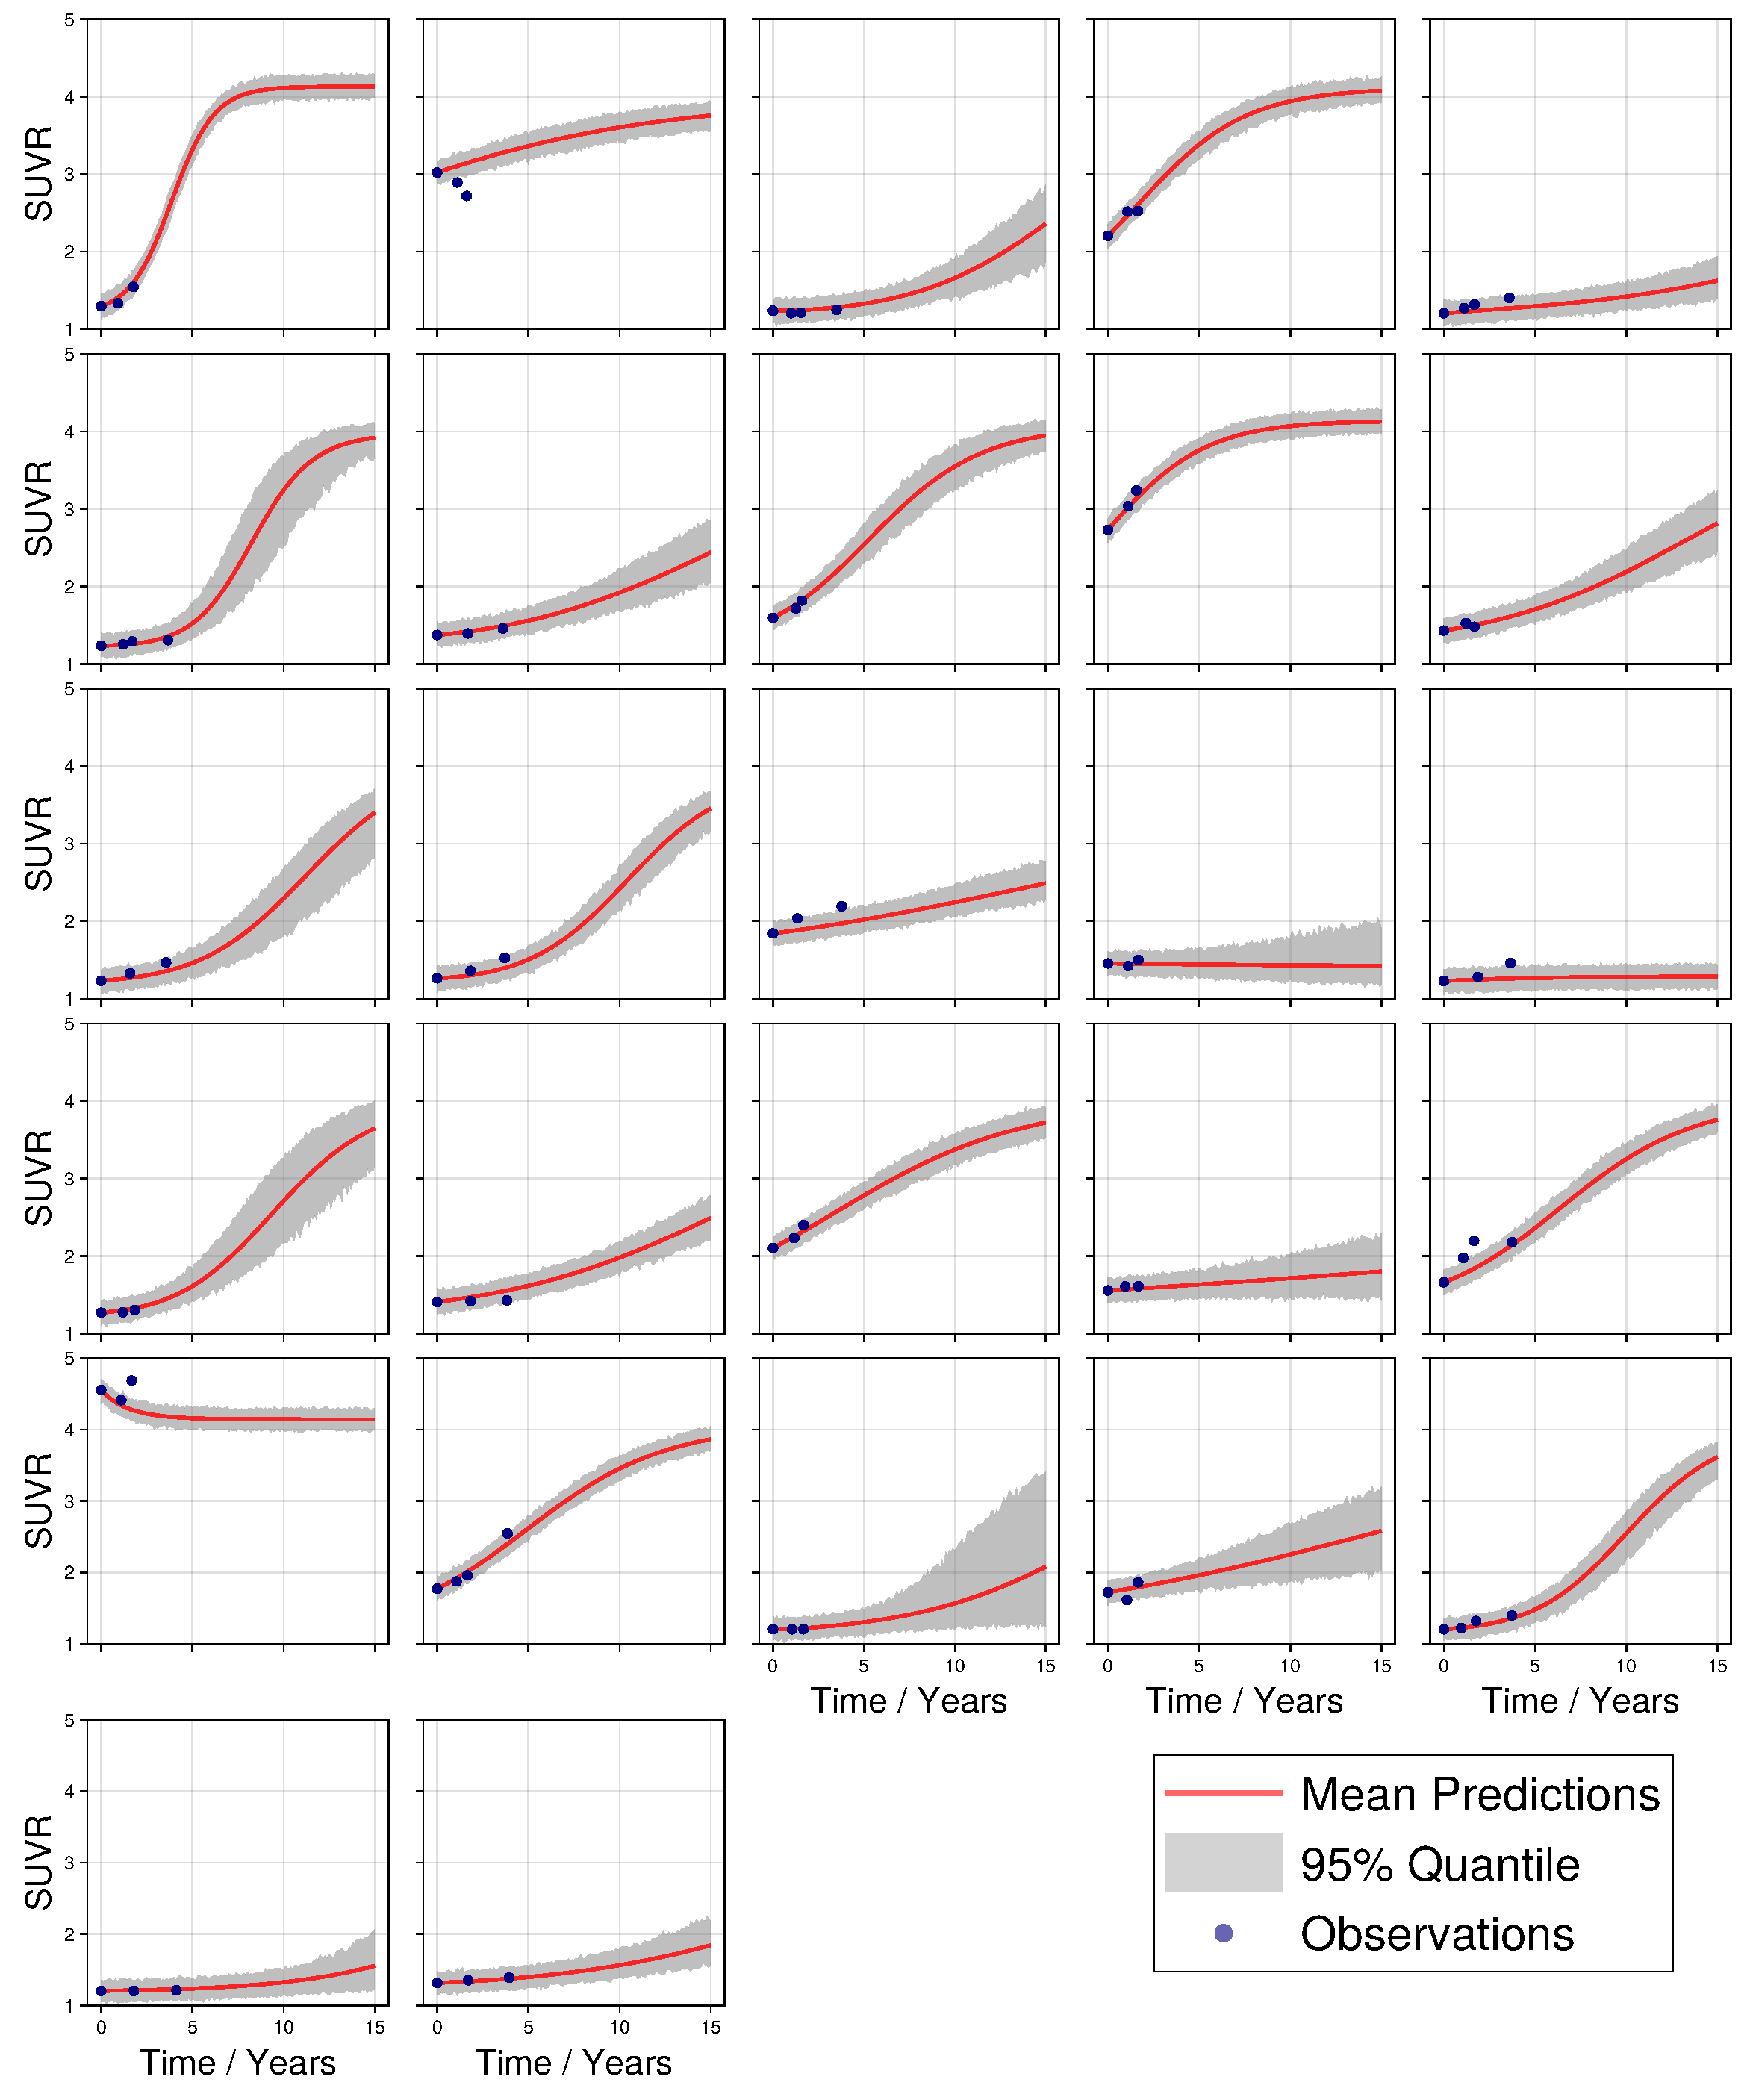
\includegraphics[width=1.0\textwidth]{biofinder/pstpred-taupos-1-inferiortemporal.pdf}
        \label{fig:pstpred-taupos-it-1-bf}
    \end{subfigure} 
    \medskip
    \caption{\textbf{Posterior predictive trajectories for the right 
                     inferior temporal lobe in BF2 \ABP \TPP}.}
\end{figure}%
\begin{figure}[H]\ContinuedFloat
    \centering
    \begin{subfigure}{1.0\textwidth}
        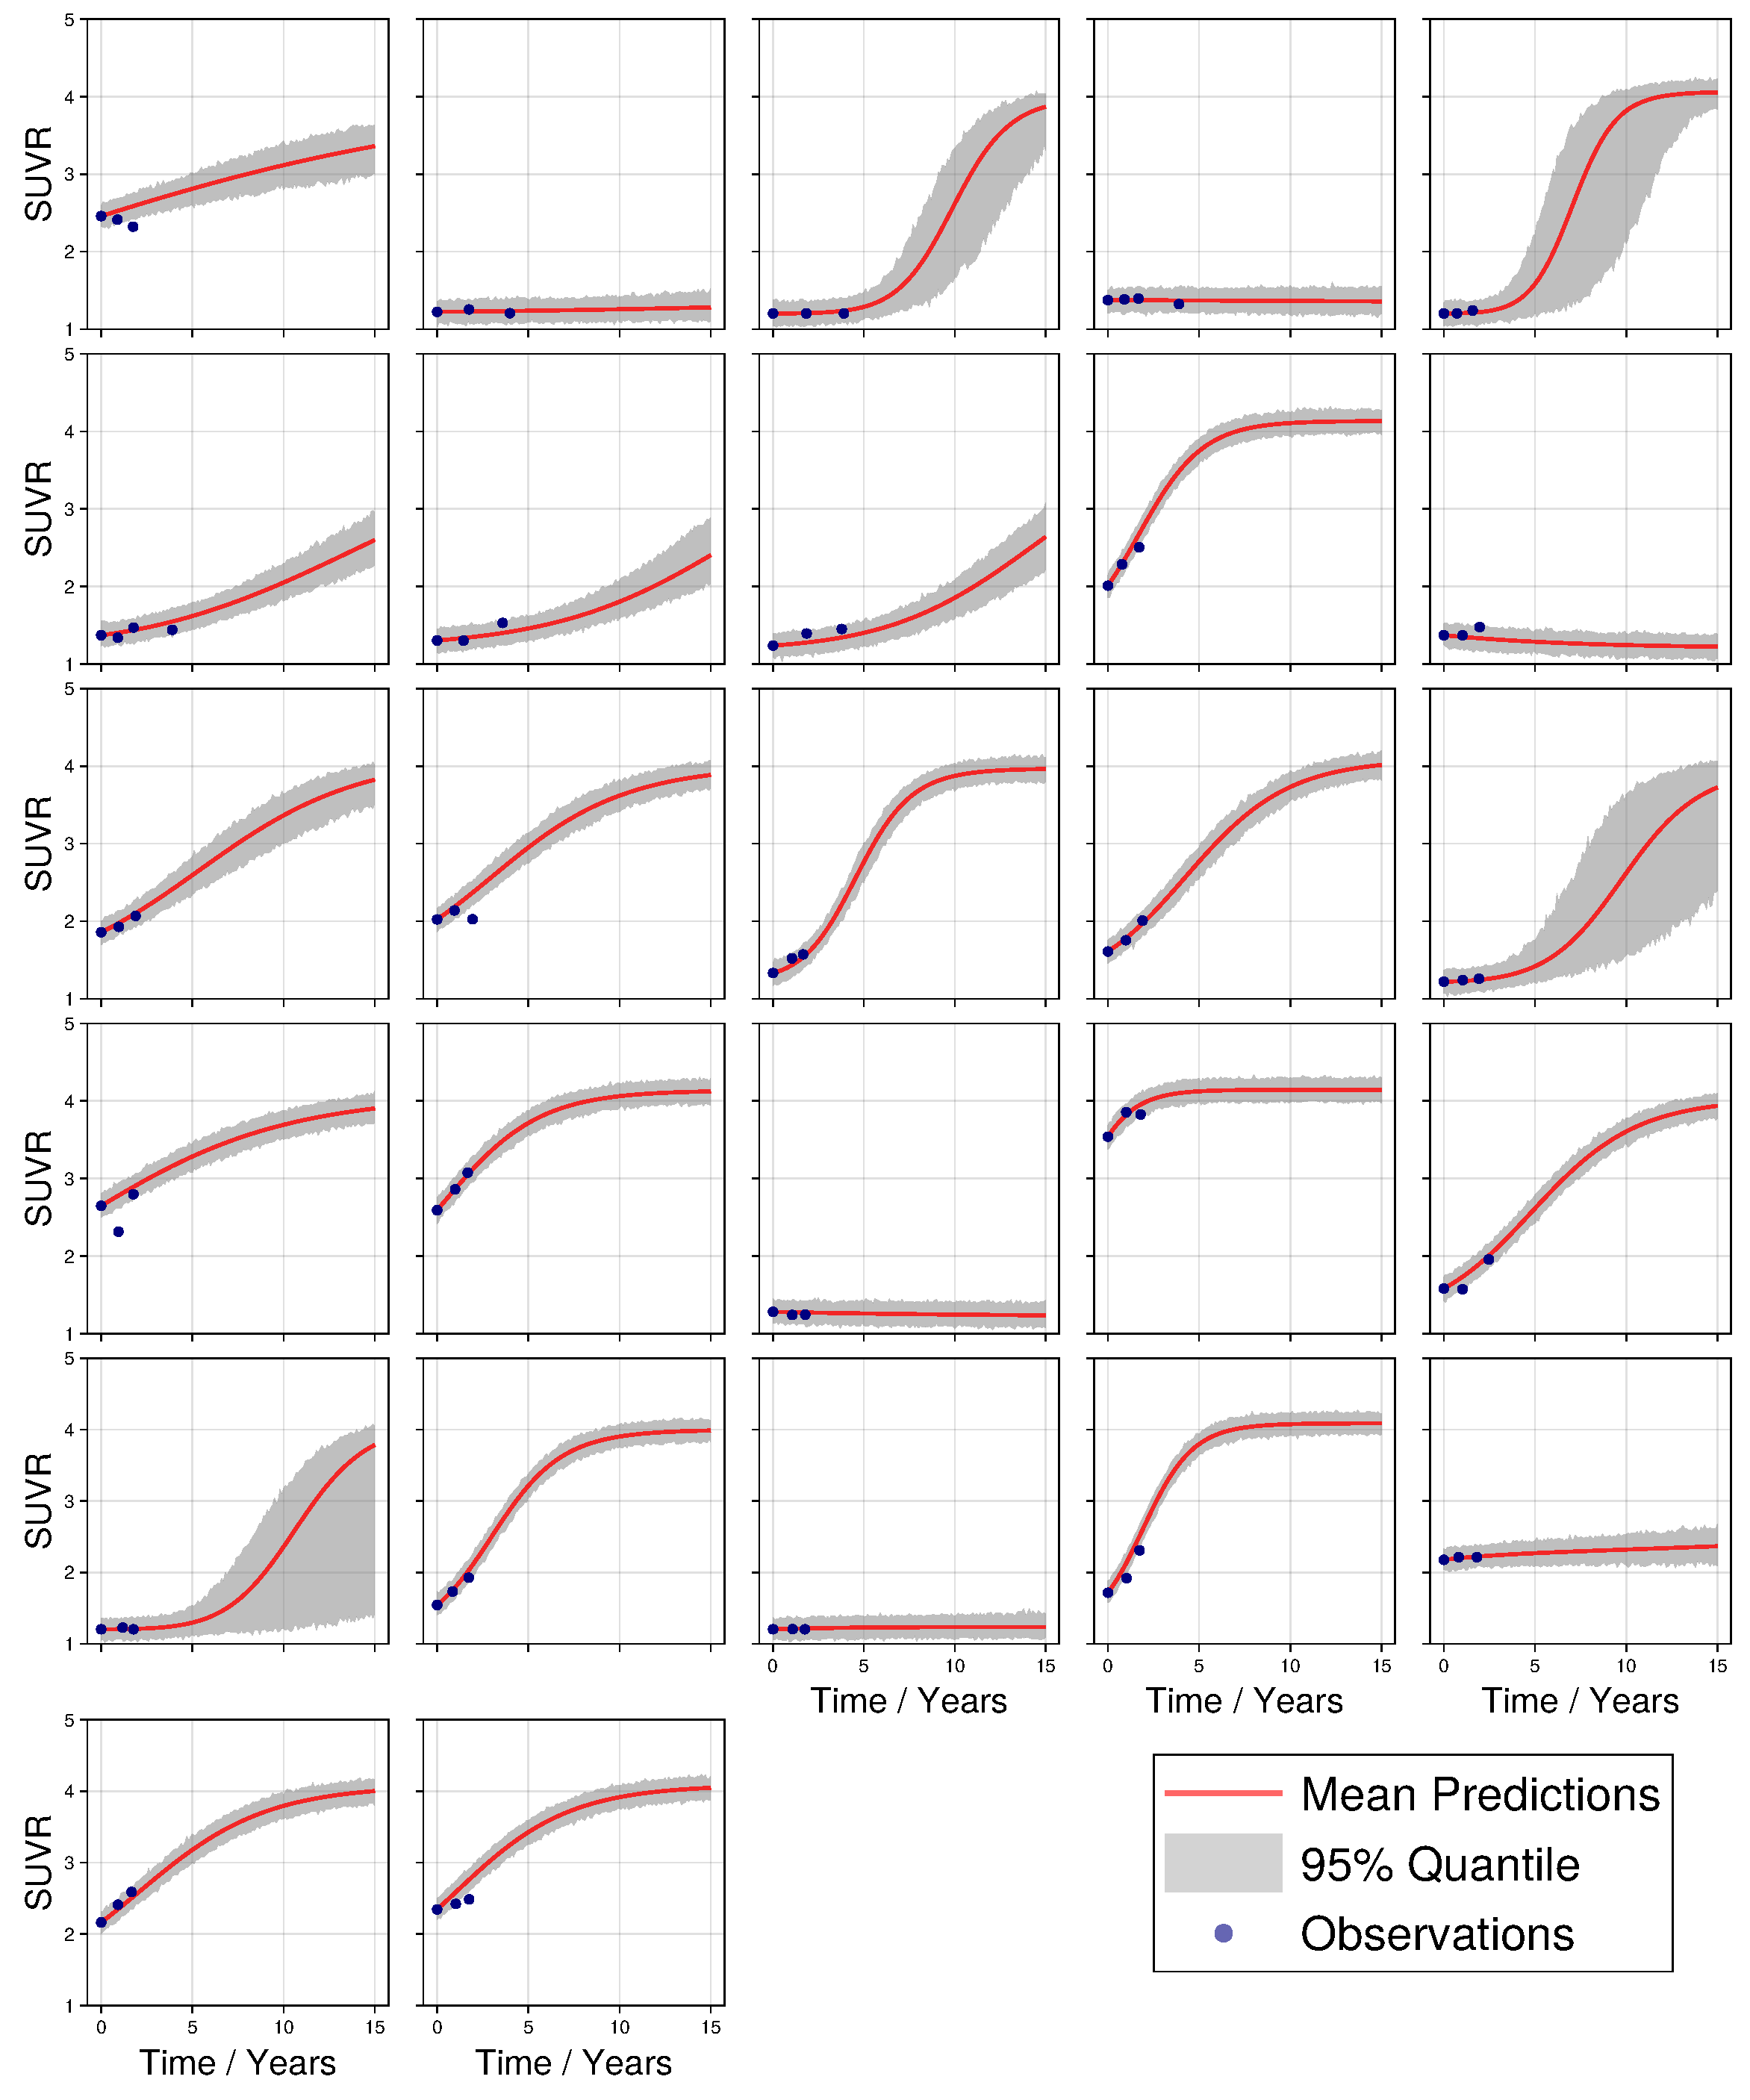
\includegraphics[width=1.0\textwidth]{biofinder/pstpred-taupos-2-inferiortemporal.pdf}
        \label{fig:pstpred-taupos-it-2-bf}
    \end{subfigure}
    \caption[]{\textbf{Posterior predictive trajectories for the right
                       inferior temporal lobe in BF2 \ABP \TPP (cont.)}
    Simulations from the posterior distributions of the BF2
    \ABP \TPP group. Shown here are data (blue scatter points) and simulated 
    trajectories (mean predictions in red and 95\% confidence intervals in grey)
    from the right inferior temporal lobe}
    \label{fig:pstpred-taupos-it-bf}
\end{figure}

\begin{figure}[H]
    \centering
    \begin{subfigure}{1.0\textwidth}
        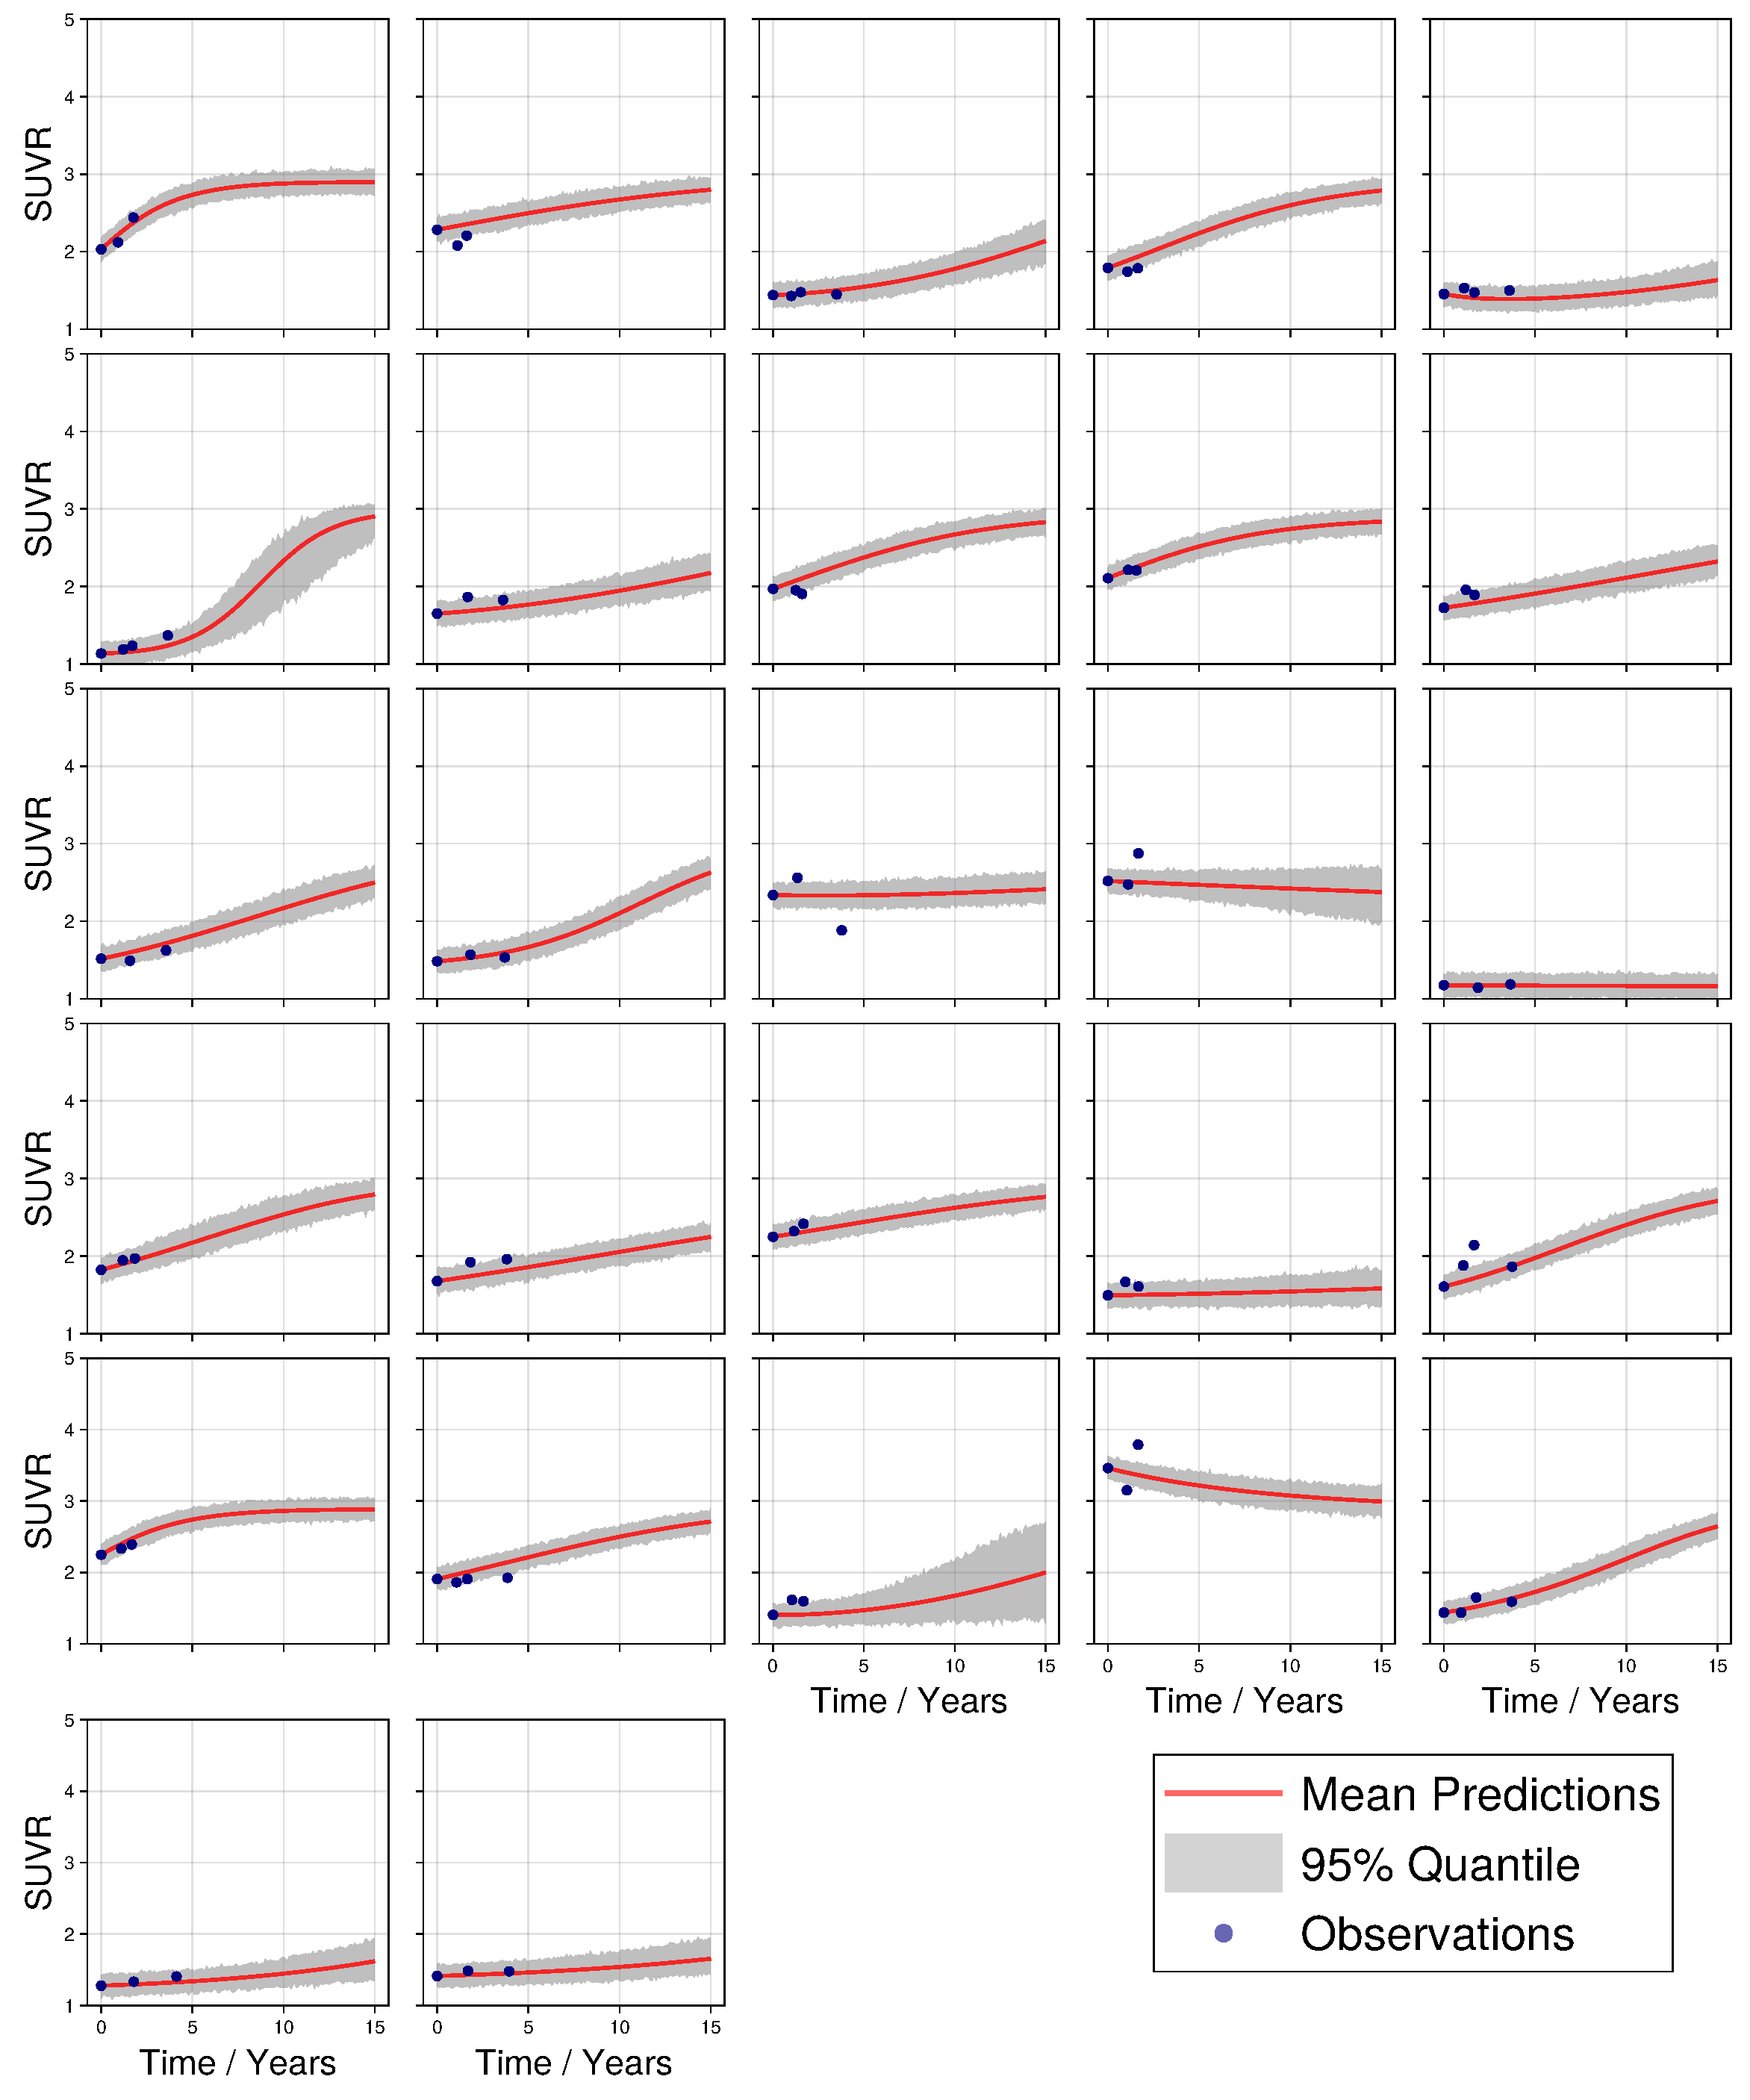
\includegraphics[width=1.0\textwidth]{biofinder/pstpred-taupos-1-entorhinal.pdf}
        \label{fig:pstpred-taupos-ec-1-bf}
    \end{subfigure} 
    \medskip
    \caption{\textbf{Posterior predictive trajectories for the right
                     entorhinal cortex in BF2 \ABP \TPP}.}
\end{figure}%
\begin{figure}[H]\ContinuedFloat
    \centering
    \begin{subfigure}{1.0\textwidth}
        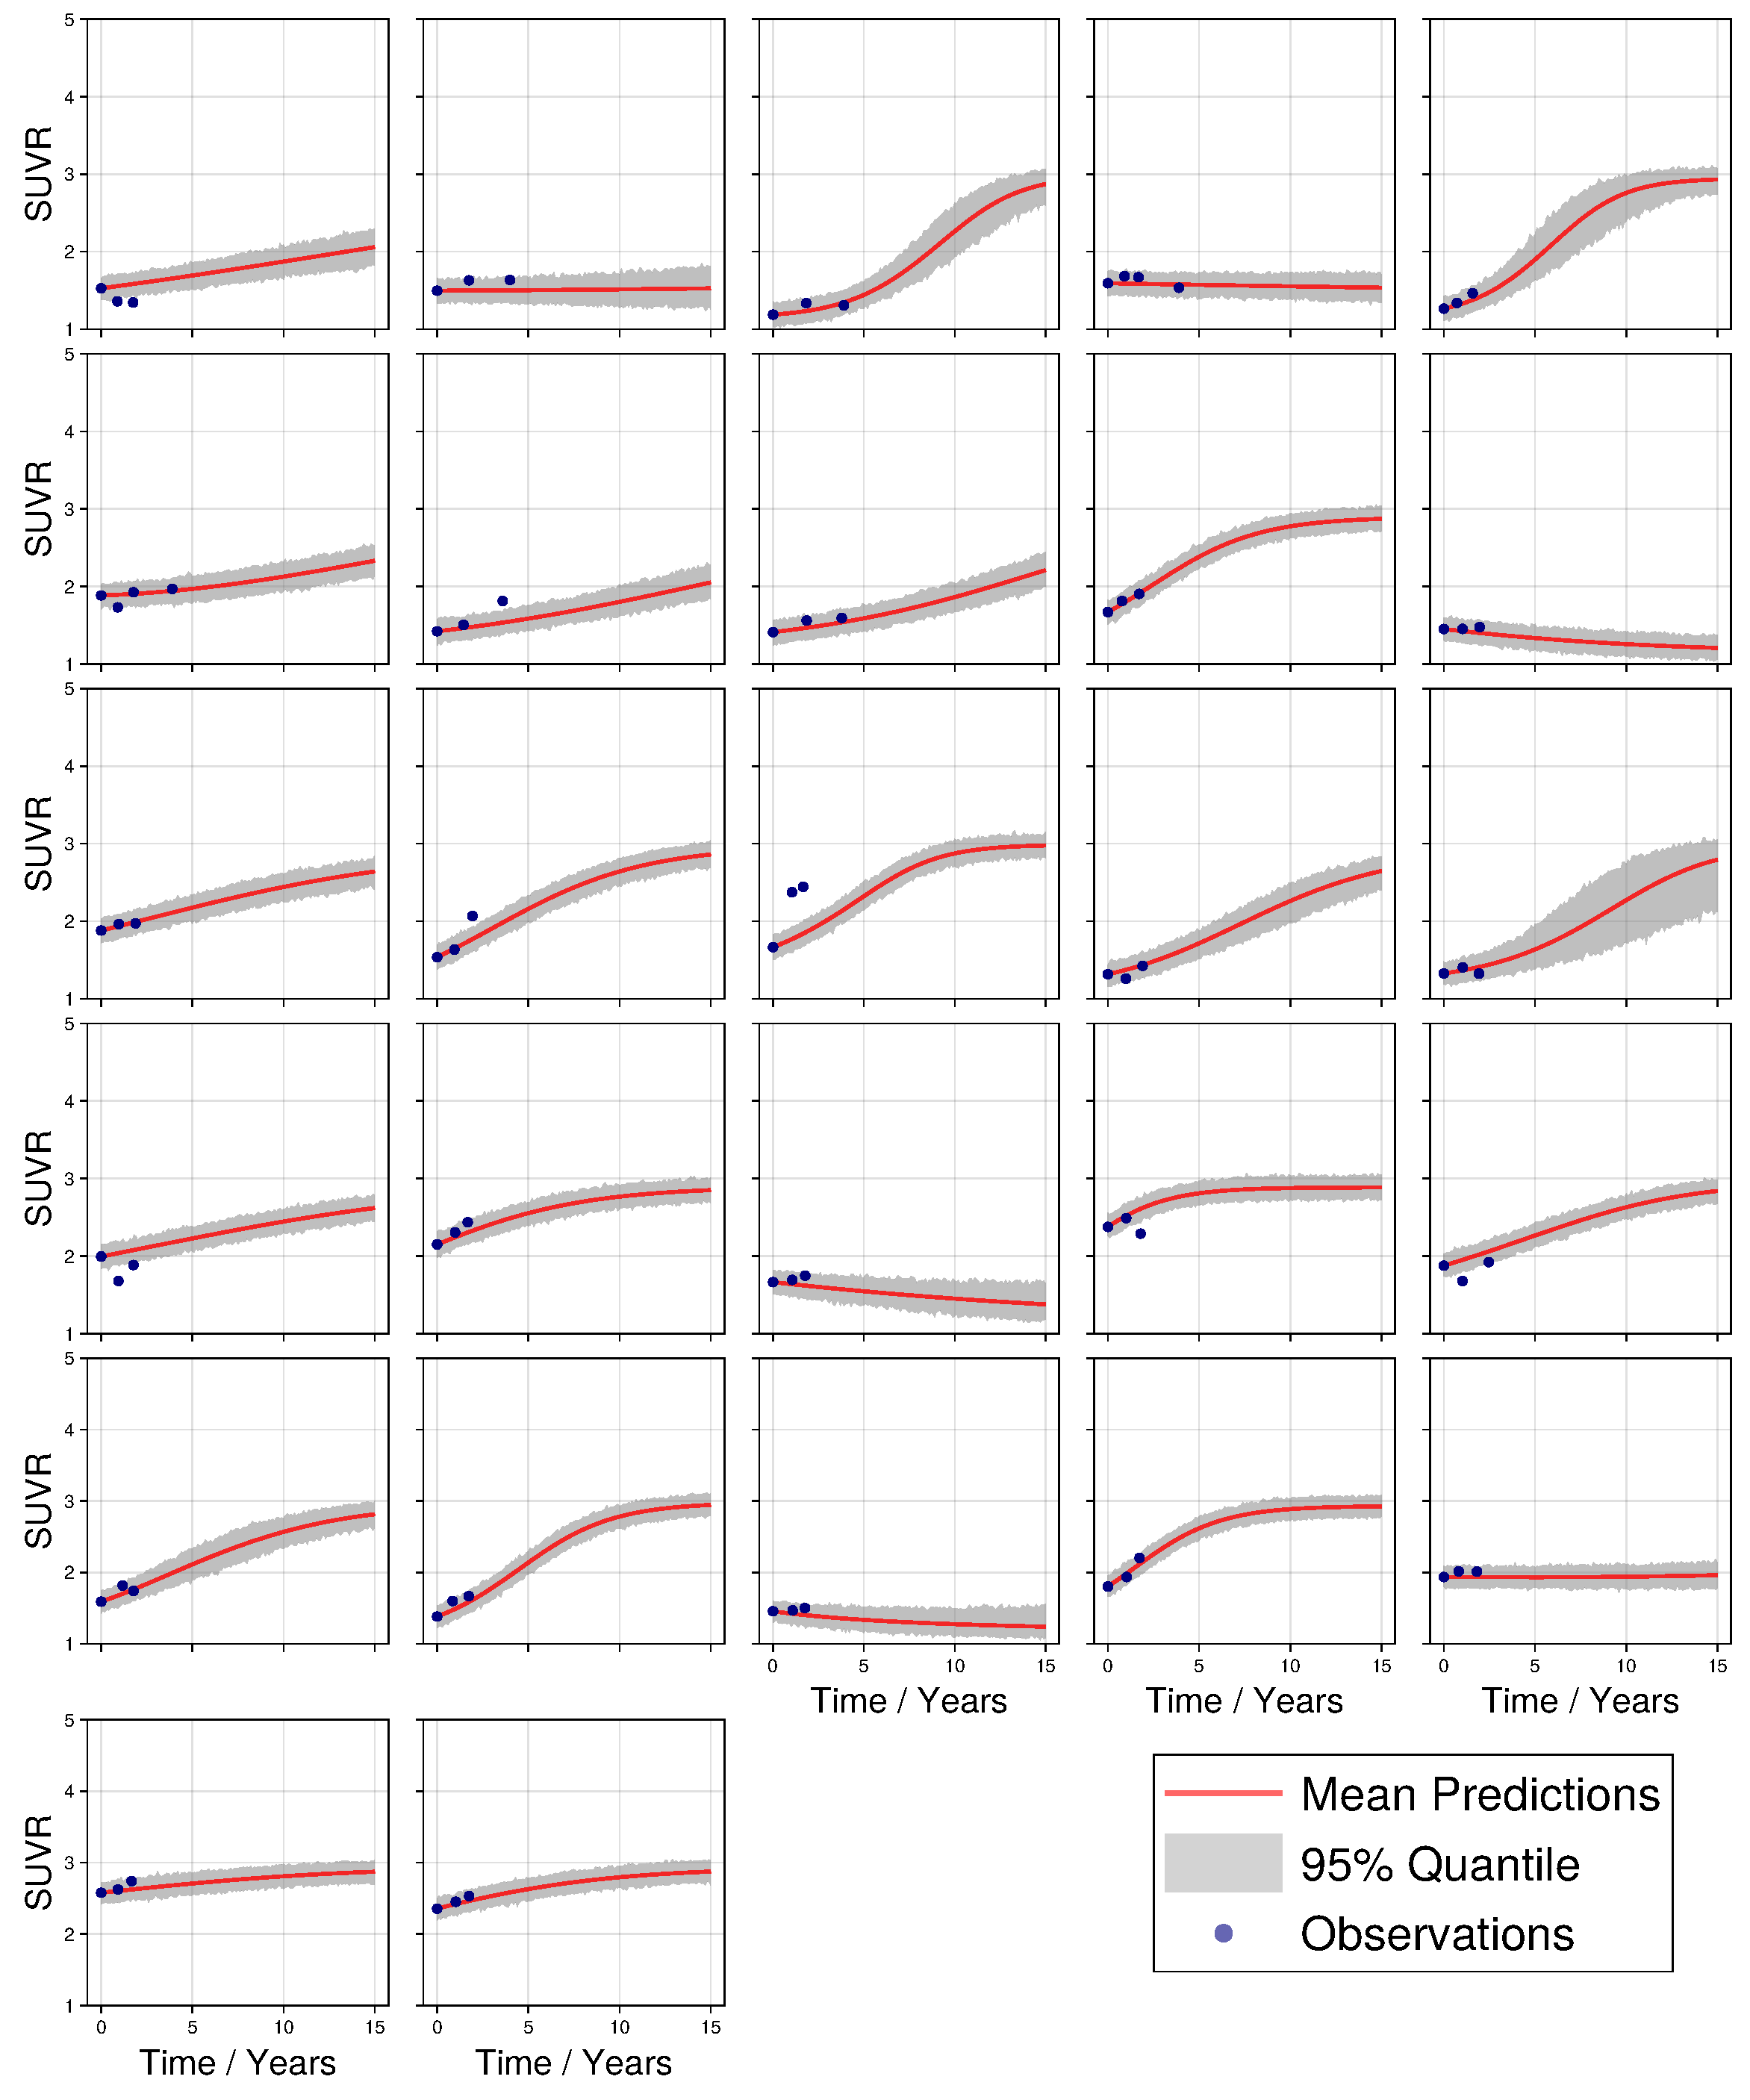
\includegraphics[width=1.0\textwidth]{biofinder/pstpred-taupos-2-entorhinal.pdf}
        \label{fig:pstpred-taupos-ec-2-bf}
    \end{subfigure}
    \caption[]{\textbf{Posterior predictive trajectories for the right
                       entorhinal cortex in BF2 \ABP \TPP (cont.)}
    Simulations from the posterior distributions of the BF2
    \ABP \TPP group. Shown here are data (blue scatter points) and simulated 
    trajectories (mean predictions in red and 95\% confidence intervals in grey)
    from the right entorhinal cortex}
    \label{fig:pstpred-taupos-ec-bf}
\end{figure}


\begin{figure}[H]
    \centering
    \includegraphics[width=1.0\textwidth]{biofinder/pstpred-tauneg-entorhinal.pdf}
    \caption{\textbf{Posterior predictive trajectories for the right
                     entorhinal cortex in BF2 \ABP \TPN}.
    Simulations from the posterior distributions of the BF2
    \ABP \TPN group. Shown here are data (blue scatter points) and simulated 
    trajectories (mean predictions in red and 95\% confidence intervals in grey)
    from the right entorhinal cortex}
    \label{fig:pstpred-tauneg-ec-bf}
\end{figure}

\begin{figure}[H]
    \centering
    \includegraphics[width=1.0\textwidth]{biofinder/pstpred-tauneg-inferiortemporal.pdf}
    \caption{\textbf{Posterior predictive trajectories for the right
                     inferior temporal lobe in BF2 \ABP \TPN}.
    Simulations from the posterior distributions of the BF2
    \ABP \TPN group. Shown here are data (blue scatter points) and simulated 
    trajectories (mean predictions in red and 95\% confidence intervals in grey)
    from the right inferiortemporal lobe}
    \label{fig:pstpred-tauneg-it-bf}
\end{figure}

\section{Discussion and Conclusions}

In this chapter, I have shown how a Bayesian framework can be used to fit a model
of \TP pathology to \TP PET data obtained from subjects across the AD spectrum.
By performing inference across different patient
groups, we have demonstrated the effects of elevated \AB and \TP levels in
patient groups, showing that subjects who are \ABN have a lower risk of disease
progression, contrasted with the higher risk group \ABP \TPN and even higher
risk \ABP \TPP group.

There have been several studies that use different kinds of computational models
to explain proteopathy in AD \cite{raj2015network, vogel2020spread}. A key
difference among the models presented in the literature are descriptions of
growth processes. For example, the diffusion model presented in
\cite{raj2012network,raj2015network} use only diffusion across the structural
connectome, whereas the epidemic spreading model presented in
\cite{iturria2014epidemic} incorporates regional growth and clearance. In this
paper, we present a parsimonious model of diffusion across the brain network and
regionally specific growth rates that relies on only two free parameters, a
global diffusion coefficient and a global protein growth rate. Using the
Gaussian mixture modelling approach to \TP PET processing presented in
\cite{vogel2020spread}, we are able to determine fixed parameters for regional
baseline values and carrying capacities, which intrinsically inform regional
growth dynamics. Our results demonstrate heterogeneity in regional growth rates,
showing that some regions are more susceptible to tau invasion and
proliferation. Additionally, our model proves to be robustly identifiable from
even limited patient data, capturing almost all variations in data within the
95\% confidence interval. 

The physical basis of the model allows for mechanistic interpretation of our
parameter inference results. Our results are consistent with experimental and
theoretical work purporting the transport of \TP through anatomical connections
\cite{liu2012trans,devos2018synaptic,vogel2020spread}. We further show that
during early stages of disease, when there is a low \TP concentration in the
medial temporal lobe, \TP dynamics are diffusion dominated but become growth
dominated later in disease. This supports previous work by Meisl et al.
\cite{meisl2021vivo} who show through an analysis of multiple datasets and
methods of \TP quantification that \TP dynamics are growth dominated from Braak
stage 3 onwards. Our results also demonstrate the growth rate of \TP increases
with the accumulation of \TP and is accelerated in later stage AD, here
characterised by the higher growth rate in \ABP \TPP compared with \ABP \TPN.
This supports data-driven work in the analysis of \TP PET showing that patients
with increased \TP burden are at higher risk of developing further AD-related
decline \cite{ossenkoppele2022amyloid}. However, due to the coarse graining
model reduction process described in \cref{sec:growth}, our model is
unable to inform about the mechanisms for increased transport in early AD and
accelerated \TP accumulation in late AD. The most likely candidate for
explaining the acceleration of \TP accumulation is the catalysing effect of \AB
on \TP templating \cite{bennett2017enhanced,he2018amyloid}. We have already 
conducted a modelling analysis of \AB and \TP interaction that displays an 
acceleration of \TP accumulation when colocalised with \AB \cite{thompson2020}.
Future work should build on this to coarse-grain the model to allow for 
inference against patient data and maintain interpretability. 

The primary contribution of this work has been to supply a parsimonious account 
of regional \TP dynamics in AD. Future work should seek to build upon this, 
adding more information and data to probe the unexplained dynamics in AD. Most 
pressingly, these include dynamical interactions between \AB and \TP in a 
sufficiently simple way to accommodate the ability to perform inference with 
patient data, i.e. not over-parametrised. Addition biomarkers of interest 
might include a coupling of \TP load with brain volume and atrophy, this would 
help account for late stage disease patients who might exhibit decreasing \TP 
concentration due to volume atrophy.